\documentclass[11pt]{scrartcl}
\usepackage[sexy]{evan}
\usepackage{graphicx}

\usepackage{answers}
\Newassociation{hint}{hintitem}{all-hints}
\renewcommand{\solutionextension}{out}
\renewenvironment{hintitem}[1]{\item[\bfseries #1.]}{}
\declaretheorem[style=thmbluebox,name={Theorem}]{thm}

 %Sets
\newcommand{\N}{\mathbb{N}}
\newcommand{\Z}{\mathbb{Z}}
\newcommand{\F}{\mathbb{F}}
\newcommand{\Q}{\mathbb{Q}}
\newcommand{\R}{\mathbb{R}}
\newcommand{\C}{\mathbb C}
\newcommand{\T}{\mathbb T}
\renewcommand{\hat}{\widehat}
\let \phi \varphi

%From Topology
\newcommand{\cT}{\mathcal{T}}
\newcommand{\cB}{\mathcal{B}}
\newcommand{\cC}{\mathcal{C}}
\newcommand{\cH}{\mathcal{H}}

\newcommand{\supp}{\text{supp }}


\begin{document}
\title{Math 222a}
\author{Vishal Raman}
\thispagestyle{empty}
$ $
\vfill
\begin{center}

\centerline{\huge \textbf{Math 222a Lecture Notes, Fall 2020}}
\centerline{\Large \textbf{Partial Differential Equations} } 
\centerline{Professor: Daniel Tataru}
\centerline{Scribe: Vishal Raman}
\end{center}
\vfill
$ $
\newpage
\thispagestyle{empty}
\tableofcontents
\newpage
%\maketitle
\section{September 1st, 2020}
\subsection{Introduction}
Partial differential equations apply to functions $u: \R^n \rightarrow \R(\C)$, where $u$ refers to the space dimension.  Usually, $n \ge 2$($n=1$ corresponds to ODEs).   

We present the following notation: \begin{itemize}
\item $\frac{\partial}{\partial x_i} u = \partial_i u$
\item There is also multi-index notation, where $\alpha = (\alpha_1, \dots, \alpha_n)$ and $\partial^\alpha u = \partial_1^{\alpha_1}\partial_2^{\alpha_2} \dots \partial_n^{\alpha_n} u$.  The size of $\alpha$ is given by $|\alpha| = \sum_{i=1}^n \alpha_i$.
\item $C(\R^n)$, continuous functions in $\R^n$.
\item $C(\Omega)$, $\Omega \subset \R^n$, continuous functions in $\Omega$.
\item $C^1(\R^n), C^1(\Omega)$, continuously differentiable functions.
\item $C^k(\R^n), C^k(\Omega)$, $k$-times differentiable.
\item $C^\infty(\R^n) = \bigcap_{k=0}^{\infty} C^k(\R^n)$.
\end{itemize}

We consider an example PDE, 
$$F(u, \partial u, \partial^2 u, \dots, \partial^k u) = 0.$$
In the above, $k \ge 1$ and $k$ is the \textbf{order} of the equation.  We also have the shorthand $F(\partial ^{\le k}u) = 0$.  

\subsection{Classification of PDE's}
\begin{definition}[Linear PDE] The PDE is a linear function of its arguments.  We can apply multi-index notation, as follows:
$$\sum_{|\alpha| < k} c_\alpha \partial^{\alpha}u = f(x).$$
If $f(x) = 0$, the PDE is \textbf{homogeneous}, otherwise it is \textbf{inhomogeneous}.
\end{definition}
This can be separated into linear PDEs with constant coefficients, $c_{\alpha } \in \R, \C$ and variables coefficients, $c_{\alpha} = c_{\alpha}(x)$.  [In this class, we focus on constant coefficient PDEs, but many of the techniques can be extended to variable coefficient PDEs.]
\begin{definition}[Nonlinear PDE]We look at a function $F = F(u, \partial u, \dots, \partial^k u)$.  The highest order terms are take the \textit{leading role}. 
\begin{itemize}
\item Semilinear PDE's: $F$ is linear, with constant or variable coefficients in $\partial^k u$: $$\sum_{|\alpha| = k} c_{\alpha}(x)\partial^\alpha u = N(\partial^{\le k-1}u).$$
The LHS is called the principal part, and the RHS is the perturbative role.
\item Quasilinear PDE's: 
$$\sum_{|\alpha|=k} c_{\alpha}(\partial^{\le k-1} u) \partial^{\alpha}u = N(\partial^{\le k-1}u).$$
\item Fully Nonlinear PDE's: $F(\partial^{\le k} u) = 0$, with a nonlinear dependence on $\partial^k u$.  
\end{itemize}
\end{definition}
Some examples:
\begin{itemize}
\item Linear, homogeneous, variable coefficients, order 1:$$\sum_{k=1}^u c_k(x)\partial_k(u) = 0.$$
\item Define $\Delta = \partial_1^2 + \dots + \partial_n^2$, the Laplacian operator.  We have a linear, constant coefficients, inhomogeneous, order 2:$$\Delta u = f.$$
\item Semilinear, order 2: $$\Delta u = u^3.$$ [Note that translation invariance makes homogeneous vs inhomogeneous not useful for classification in the case of nonlinear PDE's.]
\item Harmonic Map Equation:
$$\Delta u = u |\nabla u|^2.$$
It is still semilinear, but with a stronger nonlienarity.
\item Monge Ampere Equation:
$$\R^2, \partial_1^2 u \partial_2^2 u - (\partial_1 \partial_2 u)^2 = 0.$$
It is a fully nonlinear equation.
\end{itemize}

\subsection{Initial Value Problems}
We have various types of problems:
\begin{itemize}
\item (Stationary Problems) With $u : \R^n \rightarrow \R$,$$F(\partial^{\le k} u) = 0,$$ might describe an equilibrium configuration of a physical system.
\item (Evolution Equations) With $u : \R\times \R^n\rightarrow \R$, $u(t, x)$ describes the state at time $t$.  We can think about the order in $x$ or in $t$. 
\end{itemize}
\begin{definition}[Initial Value Problem/Cauchy Problem] A PDE with initial conditions.
\end{definition}
\begin{example} Consider the heat equation:
$$\partial_t u = \Delta_x u,$$
$$ u(t = 0, x) = u_o(x).$$
The equation is first order in $t$, but second order in $x$.
\end{example} 
\begin{example}
In $[\R \times \R]$, the vibrating string:
$$\partial_t^2 u = \partial_x^2 u,$$
$$u(t=0, x) = u_0(x),$$
$$\partial_t u(t=0, x) = u_1(x).$$
Note that this equation is second order in time, and requires 2 pieces of initial data.

An easier problem: Compute the Taylor series of $u$ at some point $(0, x_0)$. It requires $\partial_t^{\alpha} \partial_x^{\beta} u(0, x_0)$.  
\begin{itemize}
\item This is obvious if we have no time derivative or exactly 1.  
\item Second order time derivatives come from the equation.
\item Third order or higher time derivatives come from differentiating the equation:
$$\partial_t^3 u = \partial_x^2 \partial_t u.$$
\end{itemize}
\end{example}
\subsection{Boundary Value Problems}
We begin with an example.
\begin{example} Take $\Delta u = f$ in $\Omega \subset \R^3$, which represents equilibrium for temperature in a solid.  To solve, we need information about the boundary of $\Omega$.  For example,
$$\Delta u = f \in \Omega,$$
$$u = g \in \partial \Omega.$$
\end{example}
\subsection{Fluid Classification}
We take $u : \R^n \rightarrow \R(\C)$, and 
$$F(\partial^{\le k} u) =  0.$$
This is considered to be a \textbf{scalar equation}.

We could also take a \textbf{system} of equations, where $u: \R^n \rightarrow \R^m(\C^m)$, where $u = [u_i]$ a column of equations.  These are often more difficult than scalar equation.  We should have 
$$F(\partial^{\le k} u) = 0,$$
but $F : \R^{(\cdot)} \rightarrow \R^m(\C^m).$
\begin{example} A 2-system:
$$\Delta u = v,$$
$$\Delta v = -u.$$
\end{example}
We can often reduce the order of a scalar equation by turning it into a system:
\begin{example} Consider the vibrating string, $$\partial_t^2 u = \partial_x^2 u.$$
If we take $v = \partial_t u$, the it suffices to solve the system,
$$\partial_t u = v,$$
$$\partial_t v = \partial_x^2 u.$$
We van reduce it further by saying $u_1 = \partial_x u, u_2 = \partial_t u$ for the system,
$$\partial_t u_1 = \partial_x u_2,$$
$$\partial_t u_2 = \partial_x u_1.$$
\end{example}
\newpage
\section{September 3rd, 2020}
\subsection{Picard-Lindeloff Theorem}
Consider the example, $x' = f(x), x(0) = x_0$, $x: \R \rightarrow \R^n$.  We ask for existence, uniqueness,  continuous dependence on initial data.
\begin{definition}[Locally Lipschitz]
A \textbf{Lipschitz} continuous function $f$ is one that satisfies, $$|f(x) - f(y)| \le c|x-y|.$$  A function is \textbf{Locally Lipschitz} if for each $R$, there exists $c(R)$ such that 
$$|f(x) - f(y)| \le c(r)|x - y|, x, y \in \text{Ball}(0, R).$$

As examples, $f(x) = x$ is Lipschitz, $f(x) = x^2$ is not Lipschitz, but is locally Lipschitz.
\end{definition}

\begin{definition}[Locally well-posed] For each $x_0 \in \R^n$, there exists $T > 0$(lifespan) and a unique solution $u \in C^1[0, T; \R^n]$ with the property that $u_0 = x_0$ and the solution has a Lipschitz dependence on the data: $x_0, y_0$ initial data, $T = T(x_0)$.  For $T_1 < T$, there exists $\epsilon > 0$ such that if $|y_0 - x_0| \le \epsilon$ then $T(y) > T_1$ and $$\sup_{t \in [0, T_1]} |x(t) - y(t)| \le \tilde{C}|x_0 - y_0|.$$
\end{definition}
\begin{center}
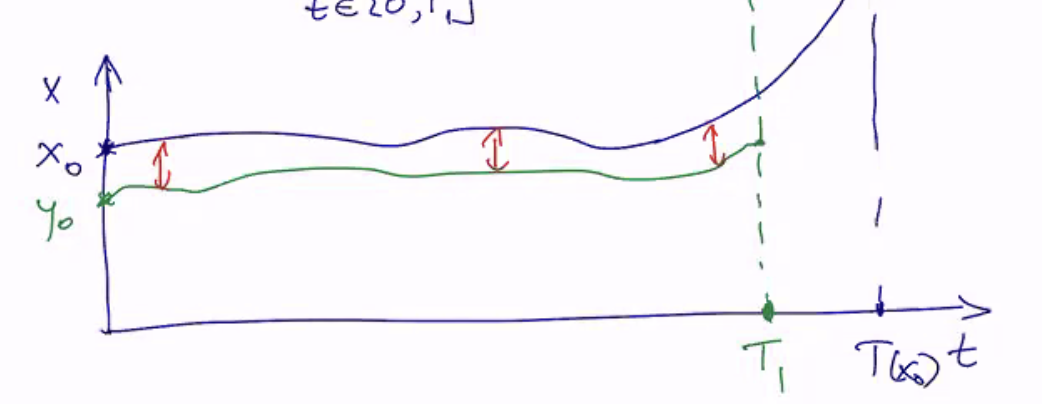
\includegraphics[scale=0.5]{localLipschitz.png}
\end{center}
\begin{thm}[Picard-Lindelof] Assume that $f$ is locally Lipschitz continuous.  Then the ODE is locally well-posed.
\end{thm}

\subsection{Contraction Principle}
We will use the "Contraction principle" - recall the following definitions:
\begin{definition}[Fixed-point Problem] Let $X$ be a Banach space,let $D \subset X$ be a closed subset of $X$, and let $F : D \rightarrow D$. Question: Can we solve the equation $F(u) = u$ where $u \in D$.
\end{definition}
\begin{definition}[Contraction] $$\|F(u) - F(v)\|_X \le L\|u - v\|,$$
where $L < 1$.
\end{definition}
If $F$ is a contraction, then it has a unique fixed point.  The existence proof follows an iterative construction: start with an arbitrary element $u_0 \in D$ and define $u_{n+1} = F(u_n)$.  We would show $\{u_n\}$ is a Cauchy sequence, so it converges.

We now prove the theorem.  We have $x' = f(x), x(0) = x_0$, so 
$$x(t) = x_0 + \int_{0}^t f(x(s))ds, t \in [0, T].$$
We choose $X = C[0, T; \R^n]$, $F(x)(t) = x_0 + \int_{0}^t f(x(s))ds.$ Then $x$ solves the ODE in $(0, T)$ if $F(x) = x$.
\begin{center}
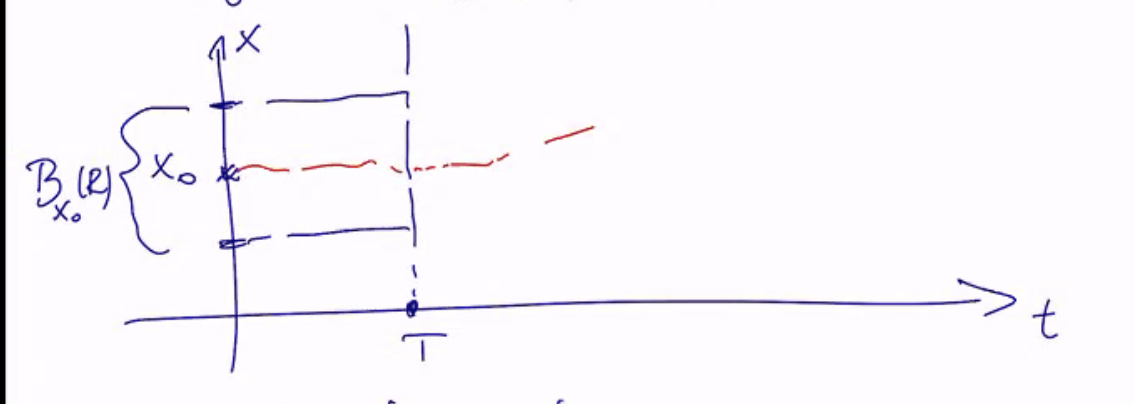
\includegraphics[scale=0.5]{ball.png}
\end{center}
We have to choose $R, T$.  Then
$$D = \{x \in X : \|x - x_0 \|_X \le R\}.$$

Let $R = |x_0|$.  Next, we choose $T$ so that $F : D \rightarrow D$ is Lipschitz.  For $F: D \rightarrow D$, we estimate the size of $F(x) - x_0$.
\begin{align*}
F(x)(t) - x_0| &= \left |\int_0^t f(x(s))ds\right | \\
&\le \left |\int_0^t f(x_0(s))ds\right | + \left | \int_0^t f(x) - f(x_0) ds \right | \\
&\le T |f(x_0)| + CT\|x - x_0\|_X  \\
\end{align*}
Hence,
$$\|F(x) - x_0\| \le T(|f(x_0)| + CR).$$
Thus, we choose $T$ such that $T(|f(x_0)| + CR) \le R$.

Now look at differences: For $x, y \in D$,
\begin{align*}
|F(x)(t) - F(y)(t)| &\le \int_{0}^t |f(x(s)) - f(y(s))| ds\\
&\le T C\sup_{s \in [0, T]} |x(s) - y(s)| \\
\end{align*}
thus,
$$\|F(x) - F(y)\|_X \le CT \|x - y\|_X,$$
so we can choose $T$ so that $CT\|x-y \|_X < 1$.

By the contraction principle, there exists a unique solution $x \in D$.  

To prove uniqueness of a solution, we have to show that any solution has to stay in $D$, up to time $T$.

\begin{center}
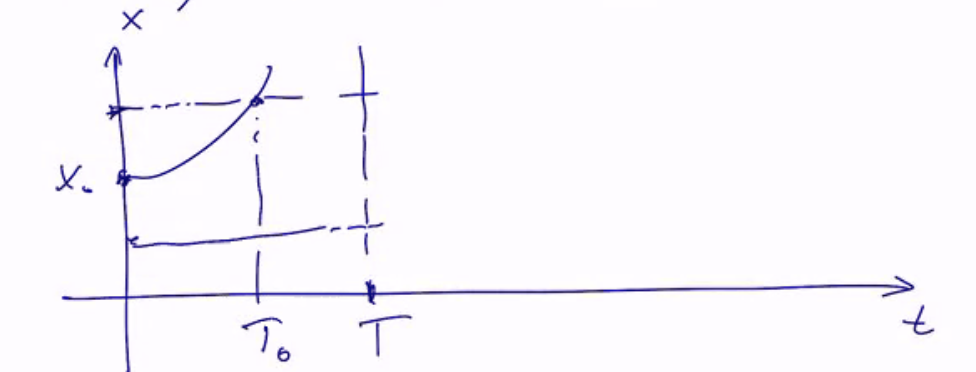
\includegraphics[scale=0.5]{unique.png}
\end{center}
Suppose a solution $\tilde{x}$ leave the ball before time $T$.  We repeat the above computation up to the exit time $T_0$.  Then, $T_0(|f(x_0) + CR|) < T$, since $T_0 < T$.  This is a contradiction since $T_0$ is the exit time.

\subsection{Bootstrap Argument}
Consider a bootstrap argument:  try to solve an equation and show that the solution $x$ satisfies some bound $\|x\|_T \le R$.  The difficulty is that a priori, we do not know any bound on $\|x\|_T$.  The solution:  make a bootstrap assumption, $\|x\|_T \le 2R$ and show that $\|x \|_T \le R$ under this assumption.  
\begin{center}
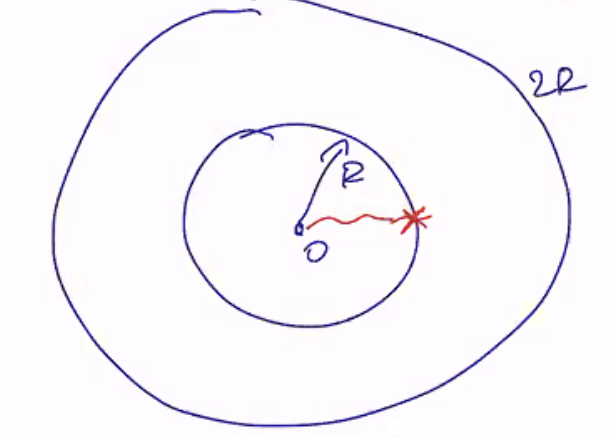
\includegraphics[scale=0.5]{bootstrap.png}
\end{center}

So far, we know uniqueness in $[0, T]$, where $T=T(x_0)$ given by the contraction argument.  We now show global uniqueness:  Suppose we have a solution $x_0$ with maximal lifespan $T_{max}(x_0)$.   Suppose $y$ is another solution.  We look at the maximal $T$ so that $x = y$ in $[0, T)$.  We now think of $T$ as the initial time.  We $x(T) = y(T)$ from continuity. Then, the solution is unique up to some time $T+T_0$, so $x = y$ in $[T, T+T_0]$, contradicting the maximality of $T$.  This is called a "continuity argument".

Next, we compare two solutions:  We have $x(0) = x_0, x: [0, T) \rightarrow R^n$.  We choose $T_1 < T$.  Then $x: [0, T_1] \rightarrow \R^n$.  We compare $x$ with a "nearby" solution $y(0) = y_0$ close to $x_0$.  We have$\|x\|_{X_{T_1}} \le R$ since we have continuity on a compact set.  We claim the following: if $|y_0 - x_0| < \epsilon$, then $x, y$ stay close.  We make a bootstrap assumption $\|y\|_{X_{T_1}} \le 2R$.  

$$\frac{d}{dt}|x-y|^2 = 2(x-y)(f(x) - f(y)) \le 2C|x-y|^2.$$

This is the \textit{Gronwall Inequality}.  It follows that $$|x-y|^2(t) \le e^{2ct}|x-y|^2(0) = e^{2ct}|x_0 - y_0|^2.$$
To close the bootstrap:
$$\|y\|_{X_{T_1}} \le \|x\|_{X_{T_1}} + \|x-y\|_{X_{T_1}} \le R + e^{cT_1}\|x_0 - y_0\| \le \frac{3R}{2},$$
which is better than the bootstrap assumption.
\section{September 8th, 2020}
Last lecture, we discussed the ordinary differential equation $x' = f(x)$ in $R^n$ with $x(0) = x_0$.  
We proved the Pircard-Lindelof theorem: if $f$ is locally Lip. then this problem is locally well-posed and the solution has a local Lip. dependence on the initial data.  We proved this by the contraction principle, using Picard iterations.
\subsection{Observations regarding Picard-Lindelof}
We note the following observations:
\begin{enumerate}
\item The result is local, so it can blow up in finite time.  

For example, take $x' = x^2, x(0) = x_0 > 0$.  The positive solutions to the ODE are $x(t) = \frac{1}{T - t}, T \ge 0$, where $T$ is the blow up time.  In this case, it is $T = \frac{1}{x_0}.$
\item If $f$ is not Lipschitz, then uniqueness might fail.

Take $x' = \sqrt{x}, x(0) = 0$.  An obvious solution is $x = 0$.  Other solutions are like $x(t) = ct^2$.  We can generate infinitely many solutions from here.
\begin{center}
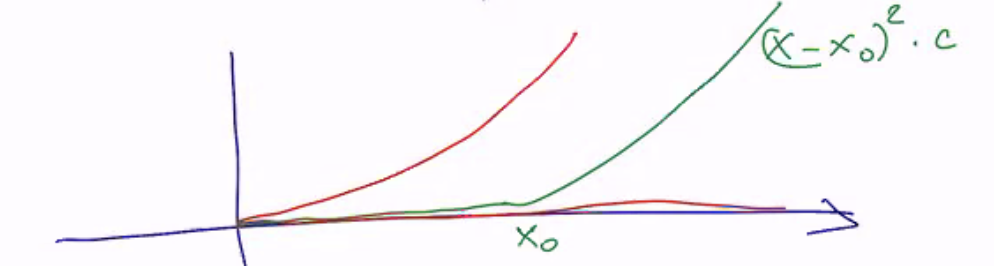
\includegraphics[scale=0.5]{notunique.png}
\end{center}
But solutions might still exist:
\begin{thm}[Peano] If $f$ is continuous, then a local solution exists.
\end{thm}
The proof uses Schauder's fixed point theorem.

\item What if $f \in C_{loc}^1$, the space of differentiable functions on a compact set?
\begin{thm} If $f \in C_{loc}^1$, then the flow map $x_0 \mapsto x(t, x_0) = \Phi(t, x_0)$ is of class $C^1$. 
\end{thm}
\begin{proof}
We give a sketch.  Take $x_0, x_0^h$ and assume $\frac{d}{dh}x_0^h(0)$ exists and show that $\frac{d}{dh}x^h$ exists.  The linearized equation about $h = 0$ is $\dot{y} = Df(x_0)y, y_0 = \frac{d}{dh}x_0^h$.  We expect that $$x^h(t) = x(t) + hy(t) + o(h).$$
Let $\tilde{x}^h(t) = x(t) + hy(t)$.  We claim that this is an "approximate solution", in the sense that $$\dot{\tilde{x}}^h(t) = f(\tilde{x}^h(t)) + o(h).$$
Furthermore, we have close initial data in the sense that
$$|x_0^h - \tilde{x}_0^h| \le o(h).$$
We repeat the difference bound for one exact and one approximate solution and show that 
$$|x^h(t) - \tilde{x}^h(t)| \le o(h)$$
\end{proof}
This implies that the Flow map is a group of local diffeomorphisms:
$$\Phi(t) \circ \Phi(s) = \Phi(t+s).$$
\end{enumerate}
\subsection{Linearization of an ODE}
The leads us to the notion of the linearization of the ODE: If we consider $x_0 \rightarrow x_0^h$, a one parameter family of data, assume this is $C^1$ in $h$.  The corresponding solution $x_0^h \rightarrow x^h(t)$ also in $C^1$ in $h$.  

What can we say about $$y^h(t) = \frac{d}{dh}x^h(t)?$$  We have $\dot{x}^h = f(x^h), x^h(0) = x_0.$  If we differentiate with respect to $h$, we have $\dot{y}^h = Df(x^h)y^h, y^h(0) = \frac{d}{dh}x_0^h.$, 
where $Df(x^h)$ is the differential of $f$, $\left (\frac{\partial f_i}{\partial x_j}\right )_{n\times m}$.   This is a linear ODE with variable coefficients.
\begin{center}
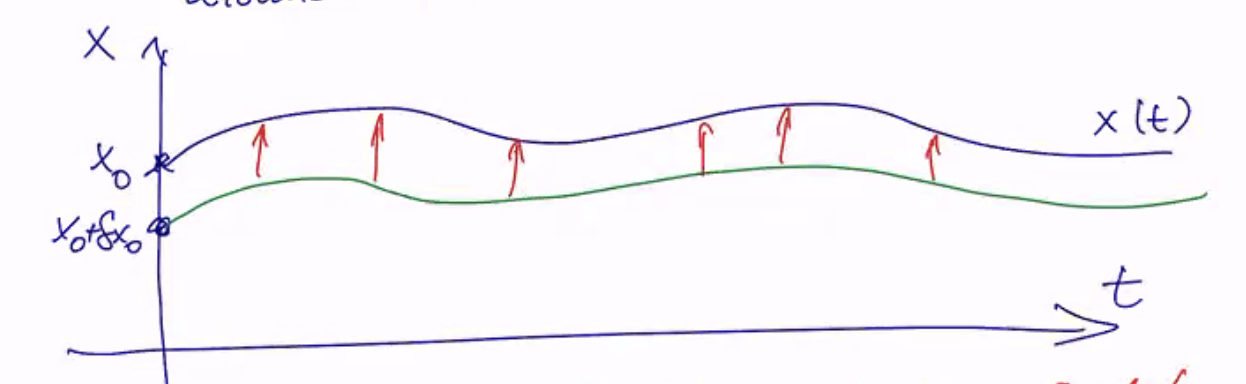
\includegraphics[scale=0.5]{linear.png}
\end{center}
\begin{proposition} If the linearized equation is well-posed, then we have Lip. dependence of solutions on the initial data.
\end{proposition}
\subsection{Our First Partial Differential Equation}
Our first example is scalar first order equations in $\R^n$, $$F(x, u, Du) = 0 \in \R^n, y:\R^n \rightarrow \R.$$
Today, we look at the case of linear, constant coefficients:
$$\sum a^i \partial_i u = f(x).$$
We will write this as $a^i \partial_i u$ following the Einstein summation convention.
Take $A = (a_1, \dots, a_n)$, so we have $A \cdot Du = f(x)$, with $A \ne 0$.  This can be interpreted as a directional derivative of $u$ in the direction $A$.
$$\frac{d}{dt}u(x(t)) = A \cdot Du(x(t)) = f(x(t)).$$
Note the fundamental theorem of calculus,
$$u(x(t)) = u(x_0) +\int_0^t f(x(t))dx.$$

Suppose we have a $C^1$ surface $\Sigma$ and we are asked to solve a $PDE$ with inidtial data $u = u_0$
 on $\Sigma$.  
 \begin{center}
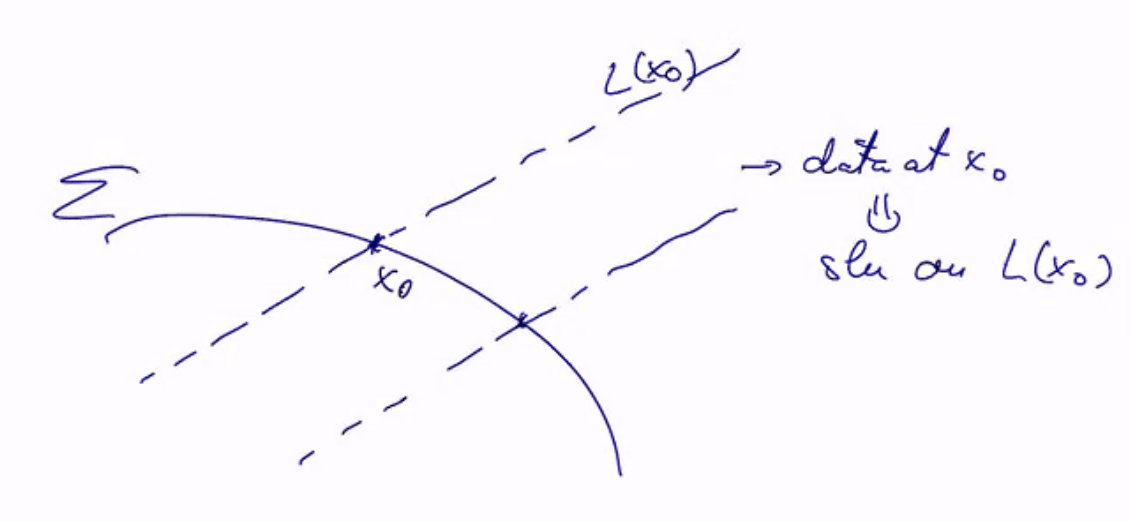
\includegraphics[scale=0.5]{sigma.png}
\end{center}
But things can go wrong.  If $\Sigma$ is a circle, we'd could have two intersection points.  Furthermore, we could miss the circle entirely and have no solutions.   Our solution in this case would be to assume that each line intersects $\Sigma$ exactly once.  However, if solutions are tangent, perturbations of the surface cause problems.  

To solve all these issues, we assume that $A$ is always transversal to $\Sigma$.  This can be written in terms of $N$, the normal vector to $\Sigma$, namely,
$$A \cdot N \ne 0.$$
\begin{definition}[Noncharacteristic Surface] If $A \cdot N \ne 0$, then we say the surface $\Sigma$ is noncharacteristic.
\end{definition}
 \begin{center}
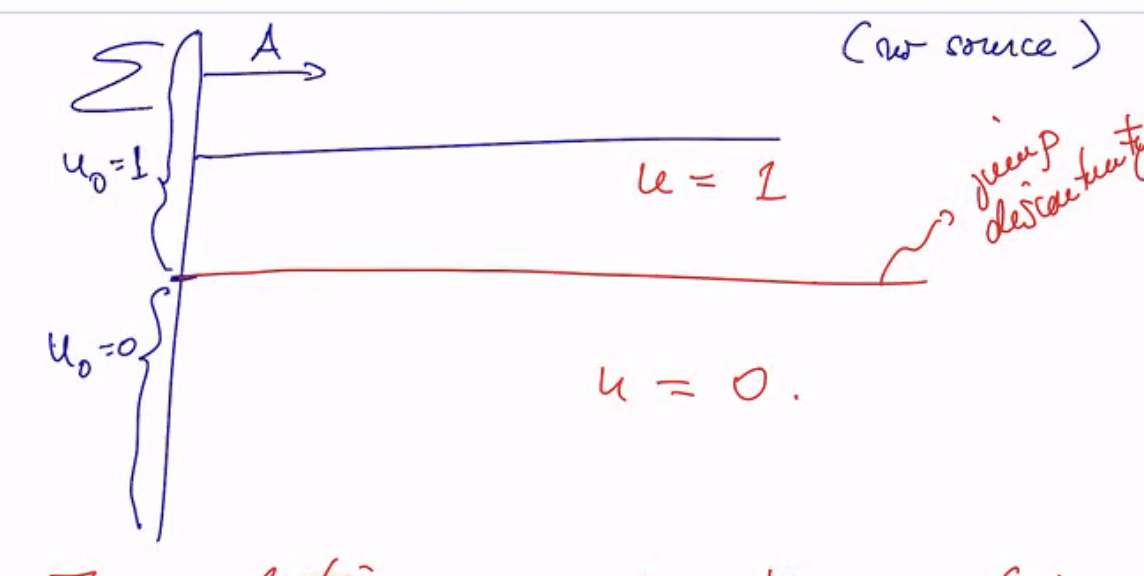
\includegraphics[scale=0.5]{bad.png}
\end{center}
We can have solutions that solve the equation at every point but not differentiable everywhere.
We learn 2 lessons from this example:
\begin{enumerate}
\item We need to enlarge the notion of what is a solution, this leads to the theory of distributions.
\item There are solutions to our PDE with a jump discontinuity along characteristic surfaces. ($\Gamma$ in the picture)
\end{enumerate}
After applying a change of coordinates, we have a Cauchy problem:
$$u_t + AD_x u = f, u(t=0) = u_0,$$
where $u_t$ is nonzero, corresponding to the condition that the surface is noncharacteristic.
\pagebreak
\section{September 10th, 2020}
Last time:
\begin{itemize}
\item We began discussing first order scalar equations.  
\begin{itemize}
\item Linear, Constant Coefficients, 
$$a^j \partial_j u = f.$$
\item We interpret the equation as a directional derivative, so solving the equation reduces to integration along straight lines.
\item For initial data, $u = u_0$ on $\Sigma$, for the problem to be well poser, we need $\Sigma$ to be \textbf{noncharacteristic}, namely 
$$A \cdot N \ne 0,$$
where $A = (a_j),$ $N$ is the normal vector to the surface.
\item Our model problem was an evolution in $(t, x),$ where $$u_t + a^j\partial_j u = f, u(t=0) = u_0.$$
\end{itemize}
\end{itemize}
\subsection{Linear, Variable Coefficients}
We have equations of the form
$$a^j(x)\partial_j u = f,$$
the \textbf{Transport equation}. 
 \begin{center}
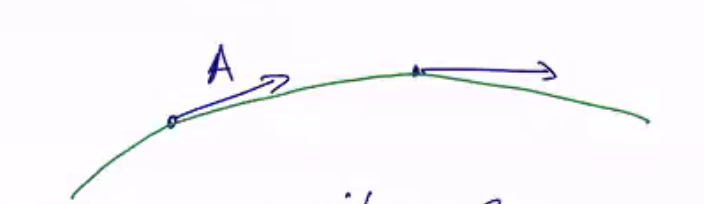
\includegraphics[scale=0.5]{curve.png}
\end{center}
Now, we have integration on curves instead of straight lines.  We think about this as ode's along curves $\gamma$ so that $A$ is tangent to $\gamma$ at every point: 
$$\dot{x} = A(x), x(0) = x_0, x(t) = \Phi(t, x_0).$$
We can rewrite this in the form
$$\frac{d}{dt} u(\Phi(t, x_0)) = f(\Phi(t, x_0)),$$
which reduces to the fundamental theorem of calculus in 2 steps:
\begin{enumerate}
\item Solve the ode
\item Integrate
\end{enumerate}
We can also add Cauchy data, $u = u_0$ on $\Sigma$.  For the problem to be well-posed, we need $\Sigma$ to be noncharacteristic, $A \cdot N \ne 0$.
 \begin{center}
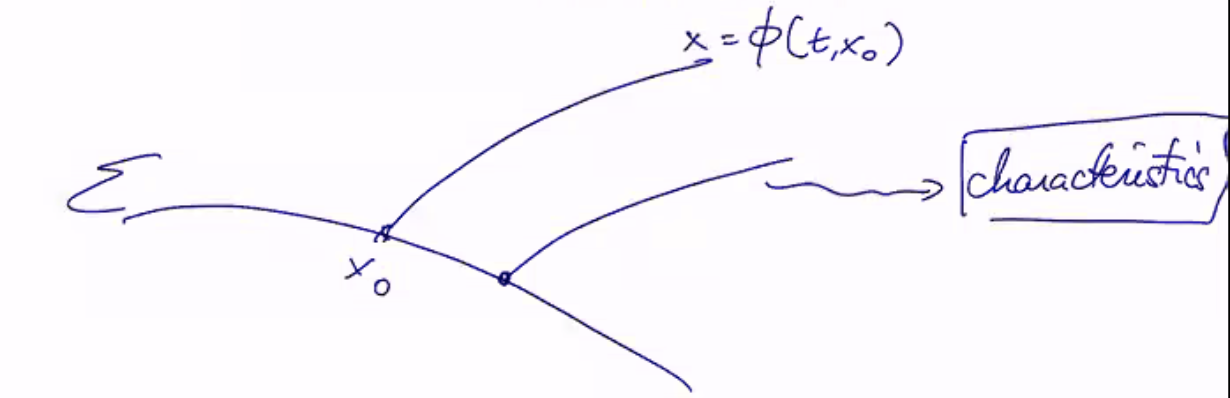
\includegraphics[scale=0.5]{char.png}
\end{center}
\begin{thm} Assume that $A \in C_{loc}^1$, $\Sigma$ is a $C^1$ noncharacteristic surface.  Then the problem
$$\begin{cases}
A \cdot Du = f  \in C\\
u = u_0 \in C \text{ on } \Sigma
\end{cases}$$
admits a unique continuous solution.
Note that if $(f, u_0) \in C$, then we can get $u \in C$ and if $(f,u_0) \in C^1$, then we can get $u \in C^1$.
\end{thm}

Having a local diffeomorphism is equivalent to showing $\Sigma$ is noncharacteristic.  We show this by showing the differential is nonzero.
 \begin{center}
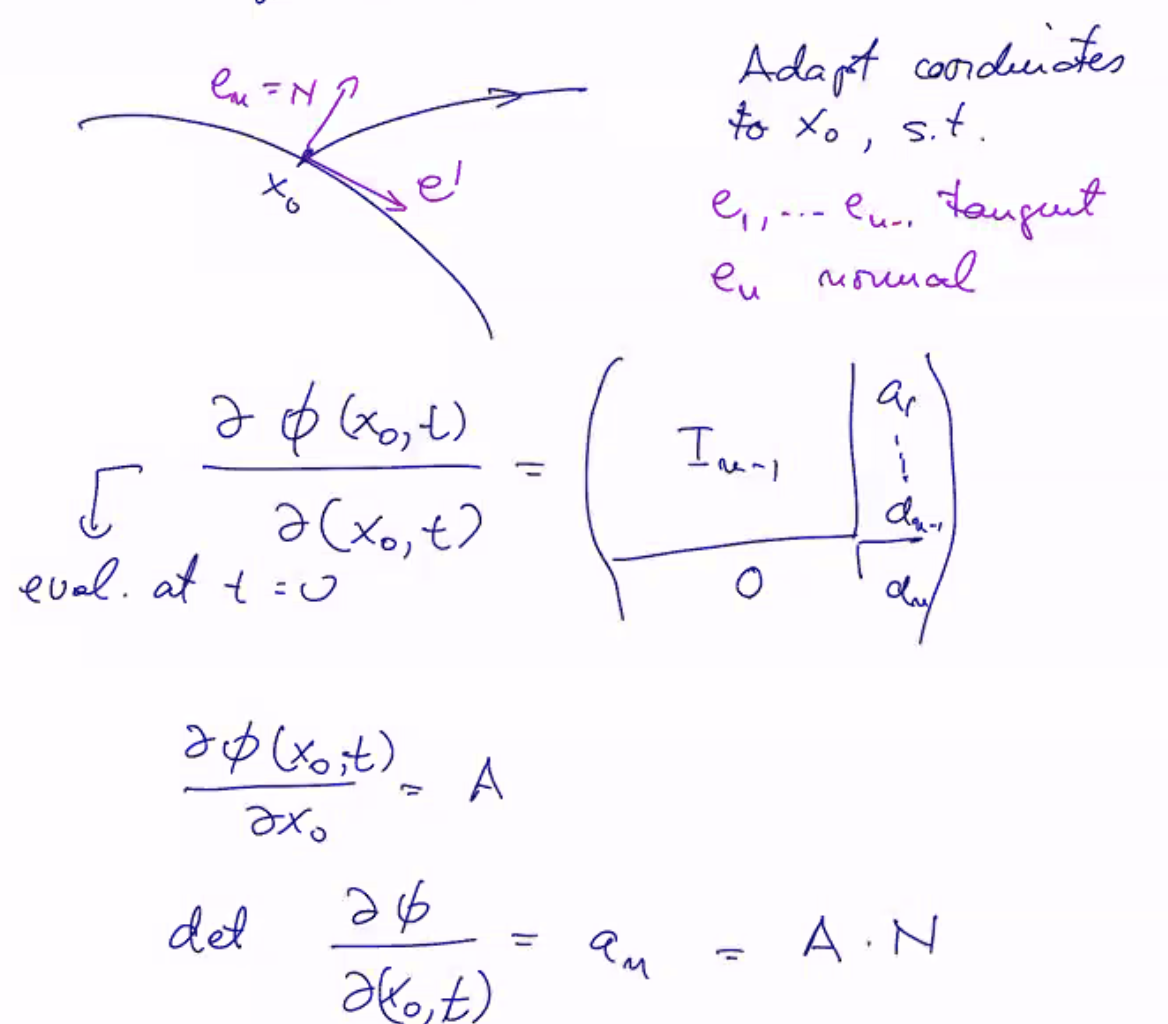
\includegraphics[scale=0.6]{diffe.png}
\end{center}
Take a change of coordinates 
$$x = \Phi(x_0, t).$$
In the new coordinates, the equation becomes
$$\frac{\partial u}{\partial t} = f, u_{t=0} = u_0,$$
which reduces completely to the fundamental theorem of calculus.
\subsection{Semilinear Equations}
We have equations of the form
$$a^j(x) \partial_j u = f(x, u).$$
We can still interpret this as a directional derivative, with an ODE:
$$\begin{cases}
x' = A(x)\\
x(0) = x_0
\end{cases}$$
with a Flow map $(x_0, t) = \phi(x_0, t)$.  We still require our surface $\Sigma$ to be noncharacteristic.

The equation along characteristics is
$$\begin{cases}
\frac{\partial}{\partial t} u (\phi(x_0, t)) = f(\phi(x_0, t), u(\phi(x_0, t)))\\
u(\phi(x_0, 0)) = u_0(x_0).
\end{cases}
$$
Then, we solve for the characteristics, and solve the ode along the characteristics.  
\subsection{Quasilinear Equations}
We have equations of the form
$$\begin{cases}
a^j(x, u)\partial_j u = f(x, u)\\
u = u_0 \text{ on } \Sigma
\end{cases}$$
A priori, we can no longer draw the vector field, since a given point will depend on the solution $u$.  

Suppose we already have a solution $u \in C^1$.  Then, we have a well-defined vector field $A = A(x, u)$.  We can also consider the flow of $A$.

 \begin{center}
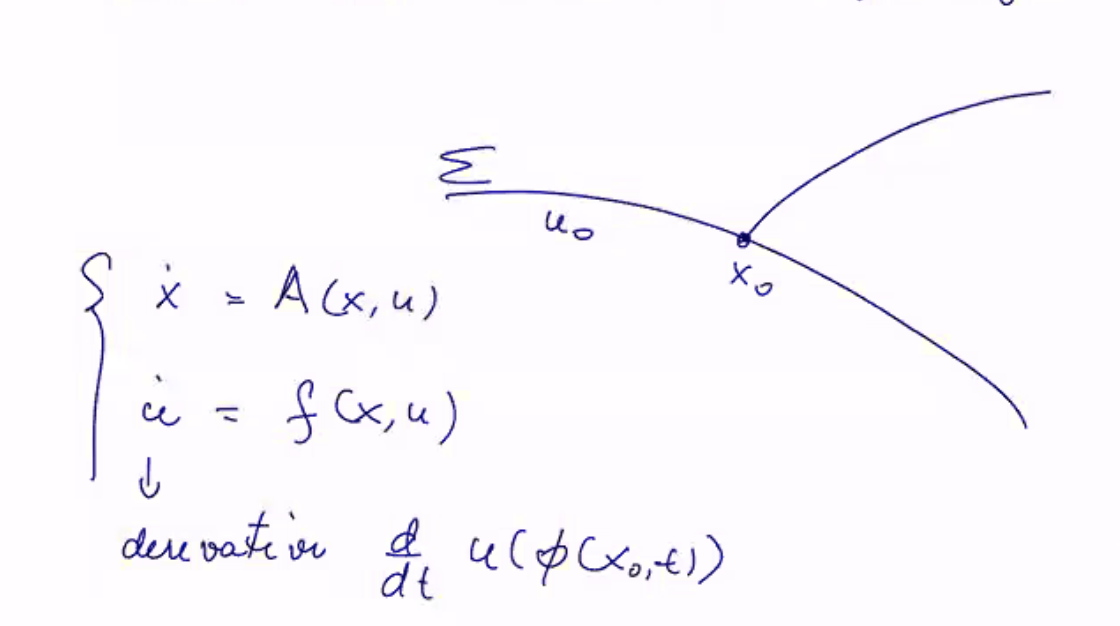
\includegraphics[scale=0.6]{quasi.png}
\end{center}
Given initial data $x(0) = x_0, u(0) = u_0(x_0)$, we have a Cauchy problem.  From this, we conclude that a good strategy for the problem is the following:
\begin{itemize}
\item Given $x_0$ on $\Sigma$, solve the above system for $x, u$.  
$$X = \phi(t, x_0, u_0), u = U(t, x_0, u_0).$$
\item Define the candidate solution $u$ as $$u(\phi(t, x_0, u_0)) = U(t, x_0, u_0).$$
\end{itemize}
Remark: We still want $\Sigma$ to be noncharacteristic: $A(x_0, u_0(x_0)) \cdot N(x_0) \ne 0$.  In this case, we say the problem is noncharacteristic, since it depends on the initial data.
\begin{thm} Let $a^j(x, u), f(x, u)$ be $C^1$ functions, $u_0 \in C^1(\Sigma)$ and $\Sigma$ noncharacteristic.  Then, the problem
$$\begin{cases}
a^j(x, u)\partial_j u = \delta(x, u)\\
u = u_0 \text{ on }\Sigma
\end{cases}$$
has a unique local solution.
\end{thm}
\begin{proof} We outline the steps.
\begin{enumerate}
\item Solve the characteristic ode:
$$\begin{cases}
\dot{x} = A(x, u)\\
\dot{u} = f(x, u)\\
x(0) = x_0 \in \Sigma \\
u(0) = u_0(x_0)
\end{cases}.$$
This gives us a local diffeomorphism:
$$(x_0, u_0(x_0), t) \rightarrow (x, u).$$
\item Define the candidate solution
$$u(\phi(x_0, u_0(x_0, t))) = U(x_0, u_0(x_0), t).$$
\item Verify that the solution is $C^1$, which comes from $C^1$ dependence for ODE's and for the local diffeomorphism.
\item Verify that the solution is unique.  [Suppose we have two solutions $u_1, u_2$ with the same initial data.   Then if their characteristic ode's have the same data, they have the same solutions, which implies that the characteristics are the same and $u_1 = u_2$ on characteristics.]
\end{enumerate}
\end{proof}
The key observation is that solutions given by the theorem are local solutions.
\subsection{Classical model problem: Burgers' Equation}
Consider the Burgers Equation: we use coordinates $(t, x) \in \R \times \R$.
$$\begin{cases}
u_t + u \cdot u_x = 0\\
u(t = 0) = u_0(x)
\end{cases}$$
 \begin{center}
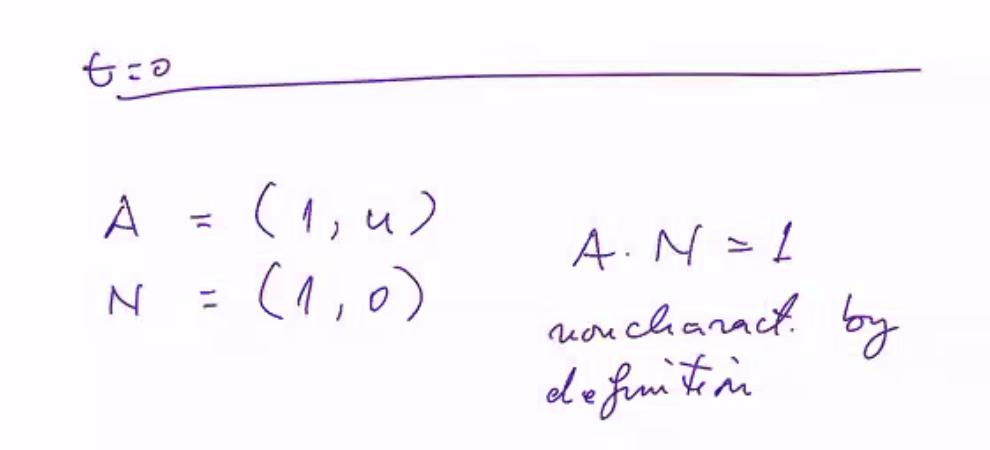
\includegraphics[scale=0.5]{burger.png}
\end{center}
If we choose a point $x_0$, the characteristic system: denote by $s$ the parameter along characteristics.  
$$\begin{cases}
\dot t = 1, t(0) = 0\\
\dot x = u, x(0) = x_0\\
\dot u = 0, u(0) = u_0(x_0)
\end{cases}$$
Our first equation is $t = s$, which tells us that $t$ is the natural parameter along characteristics.  The third equation gives us that $u = u_0(x_0)$, which is constant along characteristics.  Then, $x(t) = x_0 + tu_0(x_0)$.  In particular, characteristics are straight lines.  
 \begin{center}
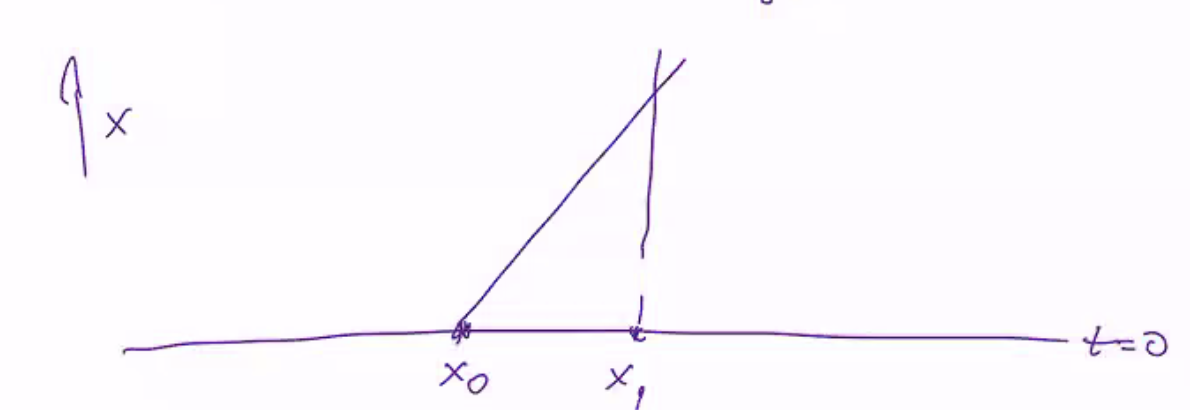
\includegraphics[scale=0.5]{intersect.png}
\end{center}
Characteristics can intersect, which loses the $C^1$ well-posedness.  To find the first $C^1$ blow-up time, we look at the first point where $x_0 \rightarrow x$ is no longer a diffeomorphism.  
$$\frac{\partial x}{\partial x_0} = 1 + tu_0'(x_0),$$
so we encounter a singularity when $tu_0'(x_0) + 1 = 0 \Rightarrow t = -\frac{1}{u_0'(x_0)}$
\pagebreak
\section{September 15th, 2020}
\subsection{Fully Nonlinear PDEs}
We have an equation $F(x, u, Du) = 0 \in \R^n$, where $Du = (\partial_1 u, \dots, \partial_n u)$.  So far, we've been able to interpret the equation as a directional derivative in the direction of $u$.  Naively, it isn't clear how to apply that approach to this system.

First, we compute the linearized equation: We have $u(h)$, a one parameter family of solutions, and take $V = \frac{d}{dh}u(h)\vert_{h = 0}.$  The $h = 0$ corresponds to the original solution.  We get that $$F_u(x, u, Du) \cdot v + F_{Du}(x, u, Du) \cdot Dv = 0.$$
We improve the notation by noting that $F: \R^n \times \R \times R^n \rightarrow \R$, and we denote $p = Du$ for convenience.  

We can rewrite the equation as 
$$F_u(x, u, Du)v + F_p(x, u, Du) \cdot Dv = F_u(x, u, Du)v + F_{p_j}(x, u, Du) \cdot \partial_j v = 0.$$

The key observation is that the linearized equation is a transport equation.  The vector field is $F_p(x, u, Du)$.  Then, we have the ordinary differential equation:
$$\dot{x}(s) = F_p(x, u, Du),$$
which are the integral curves of the vector field.  If we have a solution, we can compute it using the chain rule:
$$\dot u = F_p(x, u, Du) \cdot Du.$$
We also need $\dot{(Du)}$.  We can compute this directly with chain rule, or we can simply differentiate the original equation:
$$\frac{\partial F}{\partial x_j} + \frac{\partial F}{\partial u} \cdot \frac{\partial u}{\partial x_j} + \frac{\partial F}{\partial p_j}\cdot \frac{\partial^2 u}{\partial x_jx_k} = 0.$$
Interpreting this as a directional derivative of $\frac{\partial u}{\partial x_j}$, we have 
$$F_p \cdot D \frac{\partial u}{\partial x_j} = -F_i \cdot \frac{\partial u}{\partial x_j} - F_x,$$
$$\dot{\left (\frac{\partial u}{\partial x_j}\right )} = -F_u \frac{\partial u}{\partial x_j} - F_x.$$

We think of the three equations as a system of ODEs:
$$\begin{cases}
\dot{x} = F_p(x, u, p)\\
\dot u = F_p(x, u, Du) \cdot Du\\
\dot p = - F_u \cdot p - F_x
\end{cases}
$$
\begin{lemma} Suppose $u$ is a $C^2$ solution to our PDE.  Consider the solution to $(x, u, p)$ to the characteristic system above, with initial data $x(0) = x_0, u(0) = u(x_0), p(0) = Du(x_0)$.  Then, $$u(x(s)) = u(s),$$
$$Du(x(s)) = p(s).$$
\end{lemma}
The goal is to use this property in order to construct solutions.  

Add to the ODE an initial solution $u = u_0$ on a surface $\Sigma$.  Can we solve (locally) the initial value problem?
$$\begin{cases}
F(x, u, Du) = 0 \\
u = u_0 \in \Sigma
\end{cases}.$$
To compute characteristics starting at $x_0$, we need $x_0, u(x_0), Du(x_0)$.  We have the first two, since $u(x_0) = u_0(x_0)$.  However, $Du(x_0)$ is not immediately obvious, since $u_0$ is only on $\Sigma$, in $n-1$ variables.  In other words, we can't compute derivatives in the normal direction to $\Sigma$.  

In a frame of $x_0$ where $\Sigma = \{x_n = 0\}$,we are given $\frac{\partial u}{\partial x'} =\frac{\partial u_0}{\partial x'}$, the tangential derivatives, but not $\frac{\partial u}{\partial x_n}$.

We use the equation at $x_0$: 
$$F(x_0, u_0(x_0), Du(x_0)) = 0.  $$

We think the above as an equation for $\partial_u u(x_0)$.  Either we cannot solve it, in which case there is no solution to the PDE, or we can solve it, with some issues, namely:
\begin{itemize}
\item The solution might not be unique, in which case we make a choice that is consistent around $x_0$.
\item The outcome $\partial_n u(x_0) = G(x_0, u_0(x_0), D'u_0(x_0))$, which we want to solve smoothly. Using the "Implicit Function theorem", this happens if $\boxed{F_{p_n}(x_0, u_0(x_0), p) \ne 0}$.
\end{itemize}
\begin{thm} Consider the PDE:
$$\begin{cases}
F(x, u, Du) = 0 \\
u \vert_{\Sigma} = u_0
\end{cases}.$$
Let $x_0 \in \Sigma$, and $p_0$ so that 
\begin{itemize}
\item $F(x, u_0, p_0) = 0$
\item $p_0 \cdot T = Du_0 \cdot T$, where  $T$ is tangential
\item $F_p(x_0, u_0, p_0) \cdot N \ne 0$.
\item $F_p(x_0, u_0, p_0) \cdot N \ne 0$, the noncharacteristic condition.
\end{itemize}
(Notice that the third and fourth conditions are the same!  They come from two different places, the implicit function theorem, and our conditions on initial data.)

Then, there exists a unique $C^2$ solution of our PDE "near" $x_0$.
\end{thm}
Remark:  The solution might be only local because characteristics may intersect.

Remark: We work in $C^2$ for convenience, but the theorem holds in $C^1$.
\begin{proof}
The proof has 3 key steps:
\begin{itemize}
\item The construction of the solution.
\item The verification of the equation.
\item Verify uniqueness.
\item We would also like continuous/Lipschitz dependence on the initial data, but this part is omitted.  [It uses the linearized equation]
\end{itemize}
We begin with the construction.  We use the method of characteristics.  
$$\begin{cases}
\dot{x} = F_p(x, z, p)\\
\dot z = F_p(x, z, p) \cdot Du\\
\dot p = - F_u \cdot p - F_x
\end{cases}
$$
Find initial data for this system on $\Sigma:$ $x(0) = x_0, z(0) = u_0(x_0), p(0) = p_0$, which is obtained by solution $F(x_0, u_0(x_0), p_0) = 0$.  Recall that $p_0$ is broken into $p_T = Du_0(x_0)$ tangential, and $p_N$, normal.  We can solve this smoothly with the Implicit Function Theorem by the noncharacteristic condition.  

We solve the characteristic system with the initial data, and the outcome is a pair of functions 
$$x(s, x_0), z(s, x_0), p(s, x_0),$$
which is defined for $x_0$ is a neighborhood of the original point, $s$ in a neighborhood of $0$.

We want to define one solution $u$: We set $u(x(s, x_0)) = z(s, x_0)$.  Instead, we want $u$ as a function of $x$,
$$(s, x_0) \rightarrow x$$ needs to be invertible, i. e. a local diffeomorphism.

This equivalent to having 
$$\det \left [\frac{\partial x(s, x_0)}{\partial (s, x_0)}\right ] \ne 0,$$
which is equivalent to the noncharacteristic condition(we showed this before).  Now, we have $u$ defined in a neighborhood at $x_0$.

The next objective is to show that for $u$, we have
$$\boxed{Du(x(x_0, s)) = p(x_0, s)}.$$
We'll do this next time, but suppose we have this condition.  Then to show that $u$ solves the equation, we need that $F(x(x_0, s), u(x_0, s), p(x_0, s)) = 0$.
\end{proof}
\pagebreak
\section{September 17th, 2020}
\subsection{Fully Nonlinear PDEs, continued}
We complete the proof of the theorem from last time. 
We have functions $x(t, y), z(t, y), p(t, y)$, the solutions to the characteristic system.   They are defined in a neighborhood of $x_0$.    We also saw that the map $(t, y) \mapsto x$ is a local diffeomorphism.  Assuming we have this functions, we recall that $z$ corresponds to $u$, $p$ corresponds to $\nabla u$, so we define the candidate solution $u$ in a neighborhood of $x_0$ by setting
$$u(x(t, y)) = z(t, y).$$
This equation implies that $u$ is defined in a neighborhood, but more subtlety, it assumes that we already have a solution.  We defined $p$ in terms of $z$, so how do we know that $p$ actually corresponds to $\nabla u$?  We know that $z$ has a $C^1$ dependence on $t$ and $y$, so $p$ is a $C^1$ function.   Our objective is to show that 
$$\nabla u(x(t, y)) = p(t, y).$$

Recall, we have that $F(x_0, u_0(x_0), p_0) = 0$, so we know that on $\Sigma$, we have $p = \nabla u$, by the choice of initial data for the characteristic system.  We also know that on $\Sigma$ we have $F(x, u, p) = 0$, $u = z$ by the choice of the normal component of $p$.  

We claim that $F(x, z, p) = 0$ propagates along characteristics.  
\begin{align*}
\frac{d}{ds} F(x, z, p) &= F_x\cdot \dot x  + F_z \cdot \dot z + F_p \cdot \dot p \\
&= F_x \cdot F_p + F_z F_p \cdot p - F_p(F_z \cdot p - F_x)\\
&= 0.
\end{align*}
To prove the theorem, it remains to show that $p = \nabla u$ along each characteristic.  We would like to show that $$p_j(y, t) = \partial_{x_j}u(x(y, t)).$$

We will instead identify the derivatives of $u(x(y, t))$ with respect to $y$ and $t$.
\begin{itemize}
\item WRT $t$:\begin{align*}
\partial_t u(x(y, t)) &= \partial_{x_j}u(x(y, t)) \cdot \partial_t x_j(y, t) \\
&= \partial_{x_j}u(x(y, t))\cdot F_{p_j}(x(y, t), z(y, t), p(y, t)) \\
\end{align*}
We want this to equal $p_j \cdot F_{p_j}(x, z, p)$.  Hence, we need to show that 
$$\partial_t z(y, t) = p_jF_{p_j}(x, z, p),$$
by this is given by the characteristic equations.
\item WRT $y$:
\begin{align*}
\partial_{y_k} u(x(y, t)) &= (\partial_{x_j} u)(x(y, t)) \cdot \partial_{y_k}x_j(y, t)\\
\end{align*}
We would like this to equal $p_j(y, t) \cdot \partial_{y_k}x_j(y, t)$.  Recall that 
$\partial_{y_k}z(y, t) = p_j(y, t) \cdot \partial_{y_k}x_j(y, t)$, which is exactly what we need to show.
\end{itemize} 
Let $$r_k = \partial_{y_k}z(y, t) - p_j( y, t) \partial_{y_k} x_j(y, t).$$  We want to show that $r_k = 0$ along characteristics.  We know that $r_k = 0$ at $t=0$(on $\Sigma$).  

We will show that $r$ solves an ode:
$$\dot r = G \cdot r, r(0) = 0.$$
If this happens, then we get $r=0$.  Note that the linearization gives us equations for $\partial_{y_k} x, \partial_{y_k} z, \partial_{y_k} p$, with 
$$\begin{cases}
\dot{\left (\frac{\partial x_j}{\partial y_k}\right )} = F_{p_j x_\ell}\frac{\partial x_\ell}{\partial y_k} + F_{p_j z} \frac{\partial z}{\partial y_k} + F_{p_jp_m} \frac{\partial p_m}{\partial y_k} \\
\dot{\left (\frac{\partial z}{\partial y_k}\right )} = F_{p_j x_\ell}p_j\frac{\partial x_\ell}{\partial y_k} + F_{p_j z}p_j \frac{\partial z}{\partial y_k} + F_{p_jp_m}p_j \frac{\partial p_m}{\partial y_k}  + F_{p_j}\frac{\partial p_j}{\partial y_k}\\
\end{cases}$$
We don't actually need $\dot{\left (\frac{\partial p_\ell}{y_k}\right )}$.

Then 
\begin{align*}
\dot r_k &= \dot{[\partial_{y_k}z(y, t)]} - p_j(y, t)\dot{[\partial y_k x_j(y, t)]}\\
&=p_j \partial_{y_k}x_j(y, t)\\
&= \frac{\partial p_j}{\partial y_k} F_{p_j} - (F_z \cdot p_j + F_x) \frac{\partial p_j}{\partial y_k}.
\end{align*}
We use the fact that $F(x, z, p) = 0$ and apply $\frac{\partial}{\partial y_k}$:
\begin{align*}
0 &=F_{x_j} \frac{\partial x_j}{\partial y_j} + F_z \frac{\partial z}{\partial y_k} + F_{p_j} \frac{\partial p_j}{\partial y_k}
\end{align*}
Hence 
\begin{align*}
\dot r_k &= - F_{x_j} \frac{\partial x_j}{\partial y_k} - F_z \frac{\partial z}{\partial y_k} + (\F_z\cdot p_j + F_{x_j})\frac{\partial x_j}{\partial y_k} \\
&= -F_z\cdot \left (\frac{\partial z}{\partial y_k} - p_j\frac{\partial x_j}{\partial x_j}\right )\\
&= -F_z \cdot r_k,
\end{align*}
which gives $r=0$.

This gives existence.  For uniqueness, note that two solutions will be the same along characteristics and the characteristic equations are satisfied for $(x, u_1, Du_1), (x, u_2, Du_2)$ with the same initial data so they must coincide.

Some concluding remarks:
\begin{itemize}
\item The method of characteristics works for scalar first order equations.
\item We only get local solutions which last until characteristics start intersecting.
\end{itemize}

We have two situations where one can go further:
\begin{itemize}
\item Hamilton-Jacobi Equations:
$$\begin{cases}
u_t + H(x, D_xu) = 0\\
u(t=0) = u_0
\end{cases}.
$$The system of characteristics is 
$$\begin{cases}
\dot x = H_p \\
\dot z = H_p \cdot p \\
\dot p = -H_x
\end{cases}.$$
We can drop the middle equation for a simple pair of equations, which are the equations for Hamiltonian flows.
\item Conservation Laws:
$$\begin{cases}
u_t + F(u)_x= 0\\
u(0) = u_0
\end{cases}.
$$
Characteristics intersect in this case, which leads to jump discontinuities(shocks).  It also extends to the theory of systems.
\end{itemize}
\pagebreak
\section{September 22nd, 2020}
\subsection{Introduction to Distribution Theory}
We introduce distributions in order to generalize the solutions of equations to functions that are not everywhere differentiable. 
\begin{example}
Consider the equation
$$u_t - u_x = 0.$$
In the classic sense, we need $u$ to be differentiable.  Recall that $u(t, x) = u_0(t-x)$ solves the equation for $u_0 \in C^1$.  However, even if $u_0$ is not differentiable, we only need it to be differentiable along the directional derivative - we can call that a "generalized solution".
\end{example}

\begin{example} Let $f(x) = |x|$.  Then, $$f'(x) = \text{sgn } x = \begin{cases} -1, x < 0\\ 1, x > 0
\end{cases}.$$
\begin{center}
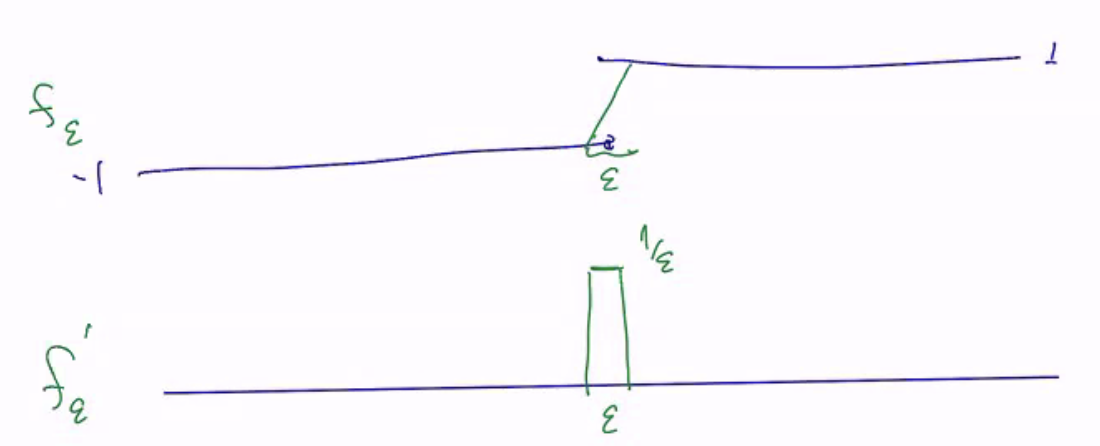
\includegraphics[scale=0.5]{images/dist.png}
\end{center}
If we approximate $\text{sgn } x$ with differentiable functions $f_\epsilon$, then as $\epsilon \rightarrow 0$, $f_\epsilon' \rightarrow 2\delta_0$, the Dirac mass at $x = 0$, which has integral 2.
\end{example}

\subsection{Frechet Space}
We can define norms on $C^k$ as follows
$$C^0 \Rightarrow \|u\|_{C^0} = \sup |u|, \|u\|_{C^1} = \sup|u| + \sup|\nabla u|, \dots$$

We define the class of seminorms $$P(K, m)(u) = \|u \|_{C^m(K)},$$
with $K$ compact and $m$ an integer.  The space of seminorms is known as a \textbf{Frechet }space, or a \textbf{locally convex space}.  In a Banach space, the topology is determined by balls $B(0, \epsilon)$(note the use of translation invariance). In the case of a Frechet space, we instead have balls determined by the seminorms:
$$\left (P_{K_1, m_1} + P_{K_2, m_2} + \dots + P_{K_j, m_j}\right )(u) < \epsilon,$$
where we have finitely many $P_{K_i, m_i}$.  

Convergence in a Frechet space is given by 
$$u_j \rightarrow u \Leftrightarrow P_{K, m}(u_j - u) \rightarrow 0$$
for all $K, m$.  The is the same as saying that 
$$\partial^\alpha u_j \rightarrow \partial^\alpha u,$$
uniformly on compact sets.

\subsection{Continuous Functions with Compact Support}
\begin{definition} $x_0 \not \in \text{supp }u$ if there exists $\epsilon > 0$ such that 
$$u = 0 \in B(x_0, \epsilon).$$
\end{definition}
\begin{example}
Consider the function $$u(x) = \begin{cases} 1-x^2, x \in [-1, 1] \\ 0, \text{ otherwise}
\end{cases}.$$
The support of $u$ is given by $[-1, 1]$.  Note that support is closed, which follows from the fact that the complement is open.  
\end{example}
\begin{fact} $\supp u$ is closed.
\end{fact}
\begin{proof}If $x_0 \not \in \supp u$ then $u=0 \in B(x_0, \epsilon)$ and for $y \not \in B(x_0, \epsilon)$, we can find $\delta > 0$ such that $u = 0 \in B(y, \delta)$.  Hence, for $u \in C(\R^n), \supp u = \overline{\{x: u(x )\ne 0\}}.$
\end{proof}

Consider the space $C_0^\infty, C_0^{\infty}(\R^n) = \mathcal{D}$, the space of continuous functions with compact support.  This is a linear space, but it's not clear that the space is nonempty.

\begin{example} The function $$f(x) = \begin{cases} e^{-1/x}, x > 0 \\ 0, x \le 0 \end{cases},$$
is a continuous function with support $[0, \infty)$.  It is not clear that the function is infinitely differentiable though.  But, we can take $f(x)f(1-x)$, a function with support in $[0, 1]$.

\end{example}

\begin{fact} If $O \subset \R^n$ is an open set, then there exists $f \in C^{\infty}(\R^n)$ such that $\supp f = \overline{O}$. This follows from Urysohn's lemma.
\end{fact}

What topology do we put on $\mathcal{D}$?  

\begin{definition}[Convergence in $\mathcal{D}$] We let $u_m \rightarrow u$ in $\mathcal D$ if 
\begin{itemize}
\item $\partial^\alpha u_m \rightarrow \partial^\alpha u$ uniformly
\item There exists a compact set $K$ such that $\supp u_m\subseteq K$ for all $m$.
\end{itemize}
\end{definition}

We cannot put Banach space on $\mathcal D$, since the norm cannot be well-defined in the case of $C^{\infty}$.  We also cannot put a Frechet space due to cardinality issues.  However, we can say that
$$\mathcal D = \bigcup_m \{u \in C^{\infty}: \supp u \subset B(0, m)\},$$
which is the union of locally convex spaces.  This is the \textbf{inductive limit topology}.  We will refer $\mathcal D$ as the space of \textbf{test functions}.

\subsection{The Space of Distributions}
This is related to the notion of duality in functional analysis. 

\begin{itemize}
 \item If $X$ is a Banach space, we can define $X^*$, the space of bounded linear functionals on $X$.  More precisely, if we have $$\|x^*\|_{X^*} = \sup_{\|x\|_X \le 1} |x^*(x)|.$$
 \item If $X$ is a Frechet space, $X^*$ is the space of continuous linear functional on $X$.  We can show that for any functional $x^* \in X^*$,
 $$|x^*(x)| \le c \sum_{i=1}^n P_{k_i}(x).$$
 \end{itemize} 
\begin{definition}[Space of Distributions] The space of distributions $\mathcal D'$ is the dual of $\mathcal D$, the space of test functions.  For any $f \in \mathcal D'$, $f : \mathcal D \rightarrow \R(\C)$, we require $f$ to be continuous:
$$u_n \rightarrow u \in D, f(u_n) \rightarrow f(u).$$
\end{definition}

Why can we think of distributions as generalized functions?  For $u \in C^{\infty}(\R^n)$, $v \in \mathcal D$, we can define the action
$$u(v) = \int_{R^n} u\cdot v dx.$$

This allows us to identify $C^{\infty}(\R^n)$ with a subset of $\mathcal D'$.  Note that this still works for $u \in C(\R^n)$ and for $u \in L^1(\R^n)$.  Furthermore, $u \in L_{loc}^1(\R^n)$, the functions that are integrable in any compact set.

We can conclude that $\mathcal D'$ contains all classical functions in the sense above, but also elements that are not functions.

\begin{example} For the dirac mass $\delta_0$, we have $\int \delta_0 u = u(0)$, so we can define $\delta_0(u) = u(0)$, and similarly, $\delta_x(u) = u(x)$.  This gives us $\delta_x'(u) = -u'(x)$ and 
$$\delta_x^(\alpha)(u) = (-1)^{|\alpha|}\partial^{\alpha} u(x).$$
\end{example}

\begin{example} For a function $f \in L_{loc}^1$, $\alpha$ a multiindex,
$$F(u) = \int_{R^n} f \cdot \partial^{\alpha} u dx.$$

We cannot do $\sum \int f_k \partial^{\alpha_k} u dx$, unless the $\supp f_k \rightarrow \infty$.
\end{example}

What is the topology on $\mathcal D'$?  
\begin{definition} $f_n \rightarrow f$ in $\mathcal D'$ if for every $u \in \mathcal D$, we have 
$$f_n(u) \rightarrow f(u).$$
\end{definition}
\begin{example} If $f_n = \delta_{x_n}$ with $x_n \rightarrow y$, $f_n \rightarrow f = \delta_y$. 
\end{example}
\pagebreak
\section{September 24th, 2020}
\subsection{The Space of Distributions, continued}
Recall, we had $\mathcal D$, the space of test functions, a linear topological space.  The notion of convergence is given by 
$$u_n \rightarrow u \text{ if } \begin{cases} \exists K : \supp(u_n) \subset K\\
\partial^\alpha u_n \rightarrow \partial^\alpha u
\end{cases}.$$
We also defined $\mathcal D'$ as the space of distributions, continuous functions $f: \mathcal D \rightarrow \R$.  We have $f_n \rightarrow f$ if $f_n(u) \rightarrow f(u)$ for all $u \in D$. We call this \textbf{convergence in the sense of distributions}.
\begin{example} If we have $C^0 \supset f_n \rightarrow f$ uniformly,
$$f_n(u) = \int f_n \cdot u dx.$$
Then
$$\int f_n \cdot u dx \rightarrow \int f \cdot u dx,$$
by uniform convergence.

This shows that classical convergence implies convergence in $\mathcal D'$.
\end{example}
 \begin{example} Suppose $f_n = \sin{nx}$, bounded functions.  This converges pointwise almost nowhere.  However,
\begin{align*}
\int f_n \cdot u dx &=\int u(x)\sin{(nx)}dx\\
&= \int \frac{1}{n}\cos{(nx)} \partial_x u(x)dx,
\end{align*}
so
$$\left |\int f_n\cdot u dx \right| \le \frac{1}{n} \int_k Cdx \rightarrow 0,$$
which implies that $\sin (nx) \rightarrow 0$ in $\mathcal D'$.
 \end{example}
 \begin{proposition} $\partial_x : \mathcal D \rightarrow \mathcal D$ is continuous.
 \end{proposition}
 \begin{example} We defined $\delta_0$, the Dirac mass as some limit of bump functions, $$f_\epsilon(x) = \begin{cases}
 \frac{1}{2\epsilon}, |x| < \epsilon \\
 0, \text{ else}
 \end{cases}.$$
 We have $\int f_\epsilon dx = 1$.  We can show formally that $f_\epsilon \rightarrow \delta_0$ in $\mathcal D'$.
 
\begin{align*}
f_\epsilon(u) &= \int f_\epsilon\cdot u dx\\
&= \frac{1}{2\epsilon} \int_{-\epsilon}^\epsilon u dx\\
&= \frac{1}{2}\int_{-1}^1 u(\epsilon x)dx \rightarrow u(0) = \delta_0(u)\\
\end{align*}
Remark:  The same works if we take $f_\epsilon =\frac{1}{\epsilon}\phi(\epsilon x)$ where 
$$\begin{cases}
\phi \in \mathcal D\\
\int \phi = 1
\end{cases}.$$
\end{example}
\begin{example} Take $\phi \in \mathcal D$, and define $f_n = \phi(x-n)$.  
\begin{align*}
f_n(u) &= \int f_n(x) u(x)dx \rightarrow 0,
\end{align*}
since the support of $f_n$ and $u$ are disjoint for large $n$.
\end{example}
\subsection{Properties of Distributions}
For partial differential equations, we need to be able to compute $P(x, \partial)f$ for $f \in \mathcal D'$,
$$P(x, \partial) = \sum c_\alpha(x) \partial^\alpha.$$

\begin{itemize}
\item Multiplication by functions: if we have $\phi \in C^{\infty}, f \in \mathcal D'$, what is $\phi f$?

Suppose $f$ was a function.  Then $(\phi f)(x) = \phi(x)f(x)$, so
$$\phi f(u) = \int (\phi f)udx = \int f \cdot (\phi u)dx = f(\phi u),$$
\begin{definition} For $\phi \in C^{\infty}, f \in \mathcal D'$, $\phi f(u) = f(\phi u)$.
\end{definition}
Note that the map $f \rightarrow \phi f$ is continuous in $\mathcal D'$.
\item Differentiation of distributions:  for $f \in C^1$, 
$$\partial_x f(u) = \int (\partial_x f) u dx = -\int f (\partial_x u)dx = -f(\partial_x u)$$
\begin{definition} For $f \in \mathcal D'$, $\partial_x f(u) = -f(\partial_x u).$
\end{definition}
Observe that $\partial: \mathcal D' \rightarrow \mathcal D'$ is continuous.  Furthermore, we have the Leibniz rule,
$$\partial(\phi f) = \partial \phi \cdot f + \phi \cdot \partial f.$$
\end{itemize}
\begin{example} $f(x) = |x|$, $\partial_x f = \text{sgn }x$, and 
$$\partial_x^2 f(u) = - \partial_x f(\partial_x u) = - \int \partial_x u \cdot \text{sgn }u dx = \int_{-\infty}^0 \partial_x u dx - \int_{0}^\infty  \partial_x u dx = 2 \delta_0(u).$$
We also have 
$$\partial_x \delta_0 = \partial_x \delta_0(u) = -\delta_0(\partial_x u) = -\partial_x u(0) = \delta_0'(u).$$
\end{example}
\subsection{The support of distributions}
\begin{definition} Let $f \in \mathcal D'$.  Then $x_0 \not \in \supp f$ if there exists $\epsilon > 0$ such that 
$f(u) = 0$ whenever $\supp u \in B_\epsilon(x_0)$.  
\end{definition}
Note that $(\supp f)^c$ is open, so $\supp f$ is closed.
\begin{proposition} Any closed set is the support of some distribution.
\end{proposition}
\begin{example} If we take $\delta_{x_0}, \supp(\delta_{x_0}) = \{x_0\}$. 
\end{example}
We let $\mathcal E' \subset \mathcal D'$ as the distributions with compact support.  
\begin{proposition} If $f \in \mathcal D'$ has compact support, then $f$ extends to a continuous functional $f: C^{\infty} \rightarrow \R$.  
\end{proposition}
\begin{proof}
We have $f:\mathcal D \rightarrow \R$ with compact support.  Let $\phi \in \mathcal D$, so that $f = 1$ in $B(0, 1)$.  We also define $\phi_R(x) = \phi\left (\frac{x}{R}\right)$.  Then $\phi_R \in D$ and $\phi_R = 1 \in B(0, R)$. 

Let $R \rightarrow \infty$.
$$\lim_{R \rightarrow \infty} \phi_R = 1$$ in $C^{\infty} = \mathcal E$, but not $\mathcal D$.  

Suppose we take $f \in \mathcal D'$, with compact support.  Let $c\in \mathcal E$.  Then
$$v = \lim_{\mathcal E} \phi_R v.$$
Define $f(v) = \lim_{R \rightarrow \infty} f(\phi_R v).$

Take 
$$f(\phi_{R_1}v) - f(\phi_{R_2}v) = f((\phi_{R_1} - \phi_{R_2}) v).$$
Then if $R_1 \subseteq R_2$, $\supp(\phi_{R_1} - \phi_{R_2}) \subset B(0, R_1)^c$.  Since $f$ is compactly supported,
$$f((\phi_{R_1} - \phi_{R_2}) v) = 0$$
if $R_1 \subset R_2$ are large enough.

Exercise:  Show that this definition does not depend on the choice of $\phi$.

Exercise: Show that $f: \mathcal E \rightarrow \R$ is continuous.

Exercise: Prove the converse: if $f:\mathcal E \rightarrow \R$ is continuous, then $f \in \mathcal E'$.

\end{proof}
\begin{example} Consider the PDE $(\partial_t - \partial_x) u = 0$.  Formally, any function $u(t, x) = g(t+x)$ should solve this.

Claim: let $g \in L_{loc}^1$.  Then $(\partial_t - \partial_x) u = 0$. 
\end{example}
\pagebreak
\section{September 29th, 2020}
Last time,
\begin{itemize}
\item We introduced $\mathcal{D}$, the space of test functions, which are smooth with compact support.  Then $\mathcal{E}$ denotes the smooth functions.
\item We denoted $\mathcal{D}'$, the space of distributions, and $\mathcal{E}'$, the space of compactly supported distributions.
\end{itemize}
\subsection{Regularity of Compactly Supported Distributions}
We introduced $C^k$, the set of $k$-times differentiable functions.  We call $k$ the \textbf{order of regularity}.

Fix $K \subset R^n$ compact, and consider $\mathcal D'(K)$.  To measure such distributions, we only need to consider test functions restricted to $K$,  If we consider $\mathcal{D}(2K)$, a locally convex space with seminorms $$P_\alpha(u) \sup_{2K}|\partial^\alpha u|,$$
$$P_{\le k}(u) = \sup_{x \in 2K} \sup_{|\alpha| \le K} |\partial^\alpha u(x)|.$$

If $f \in \mathcal D'(K)$, then $f$ must be controlled by finitely many seminorms.  But the seminorms are ordered in increasing order, so it suffices to consider a single index $k$.  Namely, there exists $k$ such that $f(u) \le C P_{\le k}(u).$
\begin{definition} The smallest $k$ for which the above holds gives the order of $f$, i. e. $-k$.
\end{definition}

For arbitrary distributions $f$:
$$f = \sum \chi_{j} f = \sum f_j$$
where $\chi_j$ is supported in $\{2^{j-1} \le |x| \le 2^{j+1}\}$, with $1 = \sum \chi_j$.  The supports of $f_j$ are going to infinity.  Each $f_j$ has an order $k_n$, but it is possible for $k_j \rightarrow \infty$.

\begin{example} Take $f \in L_{0}^1 \subset \mathcal D'$.  Then $\partial^k f \in \mathcal D'$.  What is the order of $\partial^k f$?

$$\partial^k f(u) = (-1)^{|k|} \int f \partial^k u dx,$$
so $$|\partial^k f(u)| \le \int |f| \sup |\partial^k u|dx \le \sup|\partial^k u| \int |f|dx.$$
Hence, the order of $\partial^k f$ is greater than or equal to $-k$.
\end{example}
\begin{example} The Dirac mass, $\delta_0$ has order $0$, since $\delta_0(u) = u(x)$ and $|\delta_0(u)| \le \sup |u|$.  Similarly, $\delta_0'$ has order $-1$, $\delta_0''$ has order $-2$.
\end{example}
\begin{thm} Any distribution $f$ in a compact set admits a finite representation
$$f = \sum_{k \in K}\partial^{\alpha_k}f_k,$$
where $f_k \in L_0^1$ and $K$ is finite.
\end{thm}
\subsection{Convolutions}
Note that $(\mathcal E, +, \cdot)$ is an \textbf{algebra}, which is a vector space under addition and is closed under the multiplication operation.

If we have two test functions $u, v \in \mathcal D$, define $$u * v (x) = \int u(y)v(x-y) dy.$$
The integral is well-defined since both functions have compact support.

We have some properties:
\begin{itemize}
\item Symmetry, $u * v = v * u$.  We see this by making a change of variables, $x-y = z$, $y = x-z$.  Then,
$$u * v(x) = \int u(x-z)v(z)dz  = v*u(x).$$
\item Suppose $u *v (x) \ne 0$.  Then, the integrand cannot be identically $0$, so there exists $y \in \R^n$ so that $u(y)v(x-y) \ne 0$.  Then $y \in \supp u$, $x-y \in \supp v$.  Then $$x = y + x-y \in \supp u + \supp v = \{a + b : a \in \supp u, b \in \supp v\}.$$

Hence, we have $$\supp u*v \subset \supp u + \supp v.$$
\item Regularity of convolutions:
$$u * v(x) = \int u(y)v(x-y)dy.$$
If we differentiate under the integral, 
$$\partial(u * v)(x) = \int u(y) \partial v(x-y)dy.$$
Hence $$\partial(u*v) = u * \partial v = \partial u * v.$$
\item The convolution of test functions is a test function: $\mathcal D * \mathcal D \rightarrow \mathcal D$.  \item Observe that for $u*v$ to be well defined, it is enough that one of them has compact support.  Hence $\mathcal D * \mathcal E \rightarrow \mathcal E$.                                       
\item For rough functions, we can extend this as $u \in \mathcal D$, $v \in L_0^1$, where 
$$u * v(x) = \int u(x-y)v(y)dy,$$
so $$|u*v(x)| \le \sup |u|\int |v|dx = \|u\|_\infty \cdot  \|v\|_1.$$
This gives the inequality,
$$\|u*v\|_\infty\le \|v\|_1 \cdot \|u\|_\infty.$$
In addition, if $u$ is smooth, then $u*v$ is also smooth, so 
$$\partial(u*v) = \partial u * v \Rightarrow \mathcal D * L_0^1 \rightarrow \mathcal D.$$
\item Associativity: $(u*v)*w = u*(v*w)$.    
\begin{proof}
\begin{align*}
(u*v)*w(x) &= \int(u*v)(y) w(x-y)dy \\
&=\iint u(z) v(y-z) w(x-y)dydz.
\end{align*}
Similarly,
\begin{align*}
u*(v*w)(x) &= \iint u(x-y)v(z)w(y-z) dydz.
\end{align*}
If we identify the corresponding arguments, the integrals are equal via a change of coordinates.
\end{proof}
\item $(\mathcal D, +, *)$ is an algebra.
\end{itemize}
\subsection{Convolution of Distributions}
Note that 
$$f*u(x) = \int f(y)u(x-y) dy = f(u(x- \cdot)),$$
hence, the RHS is well defined for any distribution $f$. 
\begin{definition} $f * u(x) = f(u(x - \cdot)).$
\end{definition}
Observe that $u(x-\cdot )$ is differentiable in $x$, so $f*u$ is differentiable and $$\partial f*u(x) = f(\partial u(x-\cdot))) = f(-\partial_y u(x-\cdot)) = \partial f(u(x- \cdot)),$$
hence,
  $$\partial_x(f * u) = f * \partial u = \partial f * u.$$
It follows that $\mathcal D' * \mathcal D = \mathcal E$.  We can also show that $\mathcal E' * \mathcal D = \mathcal D$.
\begin{example} $$\delta_0 * u(x) = \delta_0(u(x- \cdot)) = u(x).$$  In this sense, $\delta_0$ acts like the identity with respect to convolutions.

Similarly,
$$\delta_{x_0}*u(x) = u(x-x_0).$$
\end{example}
\pagebreak
\section{October 1st, 2020}
\subsection{Convolutions of Distributions, continued}
\begin{itemize}
\item Recall the convolution,
$$u * v(x) = \int u(x-y) v(y)dy,$$
which is a map from $\mathcal D \times \mathcal D \rightarrow \mathcal D$ and $\mathcal D \times \mathcal E \rightarrow \mathcal E$.  
\item We also saw that $\mathcal D' \times \mathcal D \rightarrow \mathcal E$.  Similarly, 
$\mathcal E' \times \mathcal D \rightarrow \mathcal D.$
\item Note that $\supp(u * v) \subset \supp u + \supp v$, $u * v = v * u$ and $u*(v*w) = (u*v)*w$.  This shows that we have a commutative algebra structure on $\mathcal D$.
\item $\delta_0$ is the identity with respect to convolutions, $\delta_0 * u = \delta_0$.
\item Consider $\mathcal D' * \mathcal D:$
$$f*u(x) = f(u(x - \cdot)).$$
\end{itemize}
We will continue to fully extend the notion of convolutions to distributions.  If we take $f \in \mathcal D'$ and $g \in \mathcal E'$, we expect $\mathcal D' * \mathcal E' \rightarrow \mathcal D'$, since we don't have regularity or compact support for $\mathcal D'$.  Similarly, we expect $\mathcal E' * \mathcal E' \rightarrow \mathcal E'$.
If $f, g$ were functions,
\begin{align*}
f*g(\phi) &= \int f * g(x)\phi(x)dx\\
&= \iint f(y)g(x-y)\phi(x)dxdy \\
&= \iint f(y)g(z)\phi(y+z) dydz\\
&= \int f(y)\left (\int g(z)\phi(y+z)dx \right )dy\\
&=\int f(y) g_z(\phi(y + \cdot_z)) dz \\ 
&= f_y(g_z(\phi(\cdot_y + \cdot_z))).
\end{align*}
Hence $f*g(\phi) = f_y(g_z(\phi(\cdot_y + \cdot_z)))$ for functions.  We take this as the definition for distributions.
\begin{proposition} This notion of convolution extends the notion of convolution for functions and has the same properties.

Recall that $$\partial (f*g) = \partial f * g = f * \partial g.$$
\end{proposition}
\subsection{Distributional Solutions to PDEs}
Consider constant coefficient partial differential equations:
$$P(\partial) = \sum){|\alpha| \le k} c_\alpha \partial^\alpha.$$
We would like to solve the equation $P(\partial)u = f$ in the smooth functions or in distributions: suppose we have $f \in \mathcal D'$.  Do we have a solution $u$?  This question is split into questions of existence and uniqueness(and continuous dependence, but this makes more sense to ask for nonlinear problems).

We refine the questions:
\begin{itemize}
\item For $f \in \mathcal D$, we wish to find a local solution $u$.  
\item We would like uniqueness with restricted behavior at infinity, but which requires considering the kernel of $P(\partial)$.  Consider exponential solutions, $u(x) = e^{x\cdot y}$.  Then $$\partial_j(e^{x\cdot y}) = y_je^{x \cdot y}, $$ $$\partial_x^{\alpha} = y^{\alpha}e^{x \cdot y},$$
so $$P(\partial)e^{x \cdot y} = P(y)e^{x \cdot y}.$$

Hence, $e^{x \cdot y}$ is in the kernel of $P(\partial)$ if and only if $P(y) = 0.$  In 1-d, we have finitely many roots, but in higher dimensions we have infinitely many roots.  Hence, we consider the restricted setting, with solutions which do not grow exponentially, for example, $y = i\xi$.  Then, $u = e^{ix\xi}$ is a solution if $P(i \xi) = 0$.

\end{itemize}
\subsection{Fundamental Solutions}
\begin{thm}[Malgrange-Ehrenpreis] All constant coefficient linear PDE's are solvable.
\end{thm}
We will prove the theorem after developing Fourier Anaylsis.  It uses the notion of a fundamental solution for constant coefficient linear PDE's.  We try to solve the equation $P(\partial)u = \delta_x$.  Then, we translate our solution by $x$, which uses the key property that $P(\partial)$ is invariant with respect to translations.

\begin{definition} $K \in \mathcal D'$ is a fundamental solution for $P(\partial)$ if $P(\partial) K = \delta_0$.
\end{definition}
\begin{proposition} If $K$ is a fundamental solution, then the function $$u = K*f$$ solves $$P(\partial)u = f.$$
\end{proposition}
\begin{proof}
$$P(\partial)u = P(\partial)(K*f) = P(\partial)K * f = \partial_0 * f = f.$$
\end{proof}
Remark:  This is useful for existence, but not for uniqueness.
\begin{example}
Consider $P(\partial) = \partial_x$ in $\R$.  We would like to solve $\partial_x K = \partial_0$.  Take $$K(x) = \begin{cases} 0, x < 0 \\1, x > 0 \end{cases},$$
the Heaviside Function.  More generally, we can take $K + H+c$ for some constant $c$ (which gives all solutions by HW 2.1).

If we want to solve $\partial_x u = f$, one of the solutions is given by $u = f * H$.  If $f$ is a nice function, then
$$u(x) = \int_\R H(y)f(x-y)dy = \int_{0}^{\infty}f(x-y)dy = \int_{-\infty}^x f(z)dz.$$
This recovers the fundamental theorem of calculus.

Note that 
$$f * c = \int f(y)\cdot c dy = c \int f,$$
which is a constant for compactly supported $f$.
\end{example}
In general, $K$ is not unique, even in the class of bounded functions.  

Note that $\supp H = [0, \infty)$ so $\supp f * H \subseteq \supp f + [0, \infty),$ which moves the support to the right.  Then $H$ is the unique forward solution, and $H-1$ is a backward solution.  Note that
$$(H-1) * f = \int (H-1)(y)f(x-y)dy = - \int_{-\infty}^0 f(x-y)dy = - \int_x^\infty f(z)dz.$$

Using $H$, we solve 
$$\begin{cases} \partial_x u = f \\ u(-\infty) = 0 \end{cases}$$
and with $H-1$, we solve
$$\begin{cases} \partial_x u = f \\ u(\infty) = 0 \end{cases}.$$
\pagebreak
\section{October 6th, 2020}
\subsection{Laplacians}
We have a PDE $P(\partial) u = f$ and $K \in \mathcal D'$ is a fundamental solution for $P(\partial)$ if $P(\partial)u = \delta_0$.  Then, $u = K * f$ solves the PDE.

\begin{example}[1D Laplacian] Take $P = \partial_x^2$.  We want to solve the equation $\partial_x^2 K = \delta_0$.  Then, integrating once gives $\partial_x K = H + C$, where $H$ is the heaviside function and $C$ is a constant. Integrating again, we get that $$K = \begin{cases}0, x < 0 \\ x, x > 0\end{cases}+Cx + D.$$
Note that $Cx+D$ solves the homogeneous problem.  

We have some special choices of solutions: 
\begin{itemize}
\item The forward solution: $$K = \begin{cases} 0, x < 0 \\ x, x > 0 \end{cases}.$$
\item The backward solution: $$K = \begin{cases} -x, x < 0 \\ 0, x > 0 \end{cases}.$$
\item The symmetric solution: $$K = |x|/2.$$

\end{itemize}
\end{example}
\begin{example} Let $P = \partial_x^2 - 1$.  

First, we solve the homogeneous equation: $$(\partial_x^2 - 1)K = 0.$$
The characteristic polynomial is $\lambda^2 - 1= 0$, so $\lambda = \pm 1$.  Hence, $u_{1,2} = e^{\pm x}.$

Next, we find the fundamental solution.  We solve $PK = \delta_0$.  $K$ must solve the homogeneous equation to the left and right of $0$.

$$K(x) = \begin{cases} c_1^{-}u_1 + c_2^{-}u_2, x < 0\\ c_1^{+}u_1 + c_2^{+}u_2, x > 0 \end{cases}$$
Then, $\partial_x K = K'(x) + [K(0)]\cdot \delta_0$. where $K'(x)$ is the formal derivative of the above and $[K(0)]\delta_0$ is the jump of $K$ at $0$.  Furthermore,
$$\partial_x^2 K = K''(x) + [K'(0)]\delta_0 + [K(0)]\delta_0'.$$

It follows that 
$$(\partial_x^2 - 1)K = K''(x) - K + \partial_x^2 K,$$
so $$(\partial_x^2 - 1)K = [K'(0)]\delta_0 + [K(0)]\delta_0' = \delta_0,$$
hence, $[K(0)] = 0$ and $[K'(0)] = 1$.

By adding multiples of the homogeneous solution, we can ensure that $c_1^+ = 0, c_2^- = 0$.  

Hence,
$$K(x) = \begin{cases} c_1^{-}e^{x},  x < 0 \\ c_2^{+}e^{-x}, x > 0\end{cases}.$$
Using $[u(0)] = 0$ gives $c_1^{-} = c_2^+$.  The second condition $[K'(0)] = 1$ gives $c_1^{-} + c_2^+ = 1$, so $$K(x) = \frac{e^{-|x|}}{2},$$
which decays exponentially at both ends.
\end{example}
\begin{example} We solve $P = \partial_x^2 + 1$.  The solutions to the characteristic equations are $\pm i$ so $ e^{\pm ix} = \cos x \pm i \sin x$ are homogeneous solutions.  Equivalently, we can take $\cos x$ and $\sin x$, since we take complex linear combinations.  We get $K(x) = \frac{1}{2} \sin |x|$ and we can add multiples of the homogeneous solutions.  Namely,
\begin{itemize}
\item The forward solution is $\sin x \cdot 1\{x > 0\}$.
\item The backward solution is $-\sin x \cdot 1\{x < 0\}.$
\end{itemize}
\end{example}
\section{Wave Equation in 1+1 Dimension} We solve $P = \partial_t^2 - \partial_x^2 = (\partial_t + \partial_x) (\partial_t - \partial_x).$

We introduce null coordinates: $u = t+x, v = t-x$.  Then $t = \frac{u+v}{2}, x = \frac{u-v}{2}.$  Hence,
$$\frac{\partial}{\partial t} = \frac{\partial}{\partial u} \frac{\partial u}{\partial t} + \frac{\partial}{\partial v}\frac{\partial v}{\partial t} = \partial_u + \partial t.$$
Similarly,
$$\frac{\partial}{\partial x} = \partial_u - \partial_v.$$
This implies that 
$$\partial_t + \partial_x = 2 \partial u, \partial_t - \partial_x = 2\partial v,$$
so $$P = (\partial_t + \partial_x)(\partial_t - \partial_x) = 4 \partial_u \partial_v.$$


In $(u, v)$ coordinates, we solve 
$$4 \partial_u\partial_v K = \delta_{0, 0} = \delta_{u = 0} \cdot \delta_{v = 0}.$$

We look for solutions 
$$K(u, v) = K_1(u) K_2(v).$$
Then, we solve 
$$\partial_u K_1 = \frac{1}{2} \delta_{u = 0}, \partial_v(K_2) = \frac{1}{2}\delta_{v = 0}.$$
The forward solutions($t > 0$) are $K_1 = \frac{1}{2}H(u), K_2 = \frac{1}{2}H(v)$, so $K = \frac{1}{4}H(u)H(v).$

We would like to switch this back in the $(t, x)$ coordinates.
We have $$P_{u, v} K = \delta_{0, 0},$$
and this corresponds to $$P_{x, y} K = J \delta_{0, 0} = \frac{\delta_{0, 0}}{2}.$$
where $J = \frac{\partial(x, y)}{\partial(u, v)} = \frac{1}{2}.$

Hence, the fundamental solution in $(x, y)$ is $$K = \frac{1}{2}\cdot 1_{t > x, t > -x}.$$

The solutions to the homogeneous equation are as follows: 
$$\partial_u \partial_v \phi = 0,$$
so $$\partial_v \phi = c(v)$$
and it follows that $$\phi = f(u) + g(v).$$

Going back to $x, y$ coordinates, we find out that $$\phi(x, t) = f(t + x) + g(t-x),$$
which are both solutions to transport equations, $\partial_t - \partial_x$, $\partial_t+ \partial_x$.

These solve homogeneous equations for $f, g$ differentiable, $f, g$ bounded and $f, g \in\mathcal D'$.  

How do we interpret $f(t+x)$ as a distribution in $(t, x)$?  If $f$ is a function, then 
$\tilde{f} = f(t+x)$, and 
$$\tilde f(\phi) = \int \tilde{f} \phi dtdx = \int f(t+x) \phi dtdx = \frac{1}{2}\int f(u)\phi(u, v)dudv = \int f(u) \left(\frac{1}{2}\int \phi dv\right)du = f(\hat \phi),$$
where $\hat \phi = \int \phi/2$.
\subsection{Back to Theory of Distributions}
We would like to approximations of the identity.  The idea is to approximate $\delta_0$ with smooth functions. Let $\phi \in \mathcal D$ with $\int \phi = 1$.  Then $\phi_\epsilon(x) = e^{-n}\phi(x/\epsilon)$, so the the integral is invariant.
\begin{proposition} $\phi_\epsilon\rightarrow \delta_0$ is in $\mathcal D'$.
\end{proposition}
\begin{proof}
\begin{align*}
\phi_\epsilon(u) &= \int \phi_\epsilon(x) \cdot u(x)dx \\
&= \int \phi(y) \cdot u(\epsilon y) dy \\
&\rightarrow \int \phi u(0) dy = u(0).
\end{align*}
So $\phi_\epsilon \rightarrow \delta_0$ in $\mathcal D'$  Hence $\phi_\epsilon$ is an approximation of the identity.  We can also call this a \textbf{mollifier}.
\end{proof} 
For $f \in \mathcal D'$, we define the regularizations as $f_\epsilon = f * \phi_\epsilon \in \mathcal E$.  

Note that $$\lim_{\epsilon \rightarrow 0} f_\epsilon = \lim_{\epsilon \rightarrow 0} f*\phi_\epsilon = f*\delta_0 = f$$ in $\mathcal D$. 

For $f_{\epsilon} \in \mathcal E$, $f \in \mathcal D'$ and for $f_{\epsilon} \in \mathcal D$, $f \in \mathcal E'$.

\begin{example} Consider the topology on $C_0(\R^n) = \{f : \R^n \rightarrow \R\}$ with $f $ continuous and $\lim_{x \rightarrow \infty} f(x) = 0$. 

Then $$\|f\|_{C_0} = \sup_{x \in \R^n}|f(x)|.$$
We have some properties:
\begin{itemize}
\item $f_\epsilon \rightarrow f$ is in $C_0(\R^n)$.
\item $|\partial^{\alpha} f_\epsilon| \le c_{\alpha}\epsilon^{-|\alpha|}.$
\end{itemize}

We could also consider $f \in L^p$ for $1 \le p < \infty$.  Then $f_{\epsilon} \rightarrow f$ in $L^p$.  
\end{example} 
\pagebreak
\section{October 8th, 2020}
\subsection{Homogeneous Functions}
\begin{definition} A function $f: \R^n \rightarrow \R$ is homogeneous of order $m$ if $f(\lambda x) = \lambda^m f(x)$ for $\lambda \in \R^+$.
\end{definition}
\begin{example}[Homogeneous Functions in $\R$] If $m \in \N$, the function $f(x) = x^m$ is homogeneous.  More generally in $\R$, $$f(x) = x_+^m = \begin{cases} 0, x < 0\\ x^m, x > 0\end{cases}$$ or $$f(x) = x_-^m = \begin{cases} (-x)^m, x < 0\\ 0, x > 0\end{cases}.$$
Linear combinations of these work as well.
\end{example}
\begin{example}[Homogeneous Functions in $\R^n$] We consider Polar coordinates: $x = r\Theta$ for $\Theta \in S^n$.  Then $f(x) = r^m g(\Theta)$.
\end{example}
These functions are directly distributions if they are locally integrable.  The happens in $\R^n $if $m > -n$.  For example, $\frac{1}{|x|^n}$ is not integrable(a borderline case).

Suppose $f$ is $m$-homogeneous.  Then $\partial f$ is $m-1$ homogeneous.

\subsection{Homogeneous Distributions}
Let $u_\lambda = \frac{1}{\lambda^n}u(x/\lambda)$ for $u \in \mathcal D$, $\lambda > 0$. In particular, $\int u_\lambda = \int u$.  

Consider a homogeneous function $f$ of order $m$.  Then,
$$\int f(\lambda x) u(x)dx = \lambda^m \int f(x)u(x)dx.$$
Furthermore, $$\int f(\lambda x)u(x)dx = \frac{1}{\lambda}\int f(y) u(y/\lambda)dy.$$
Therefore, $$f(u_\lambda) = \lambda^m f(u).$$
\begin{definition} A function $f$ is homogeneous of order $m$ if $f(u_\lambda) = \lambda^m f(u)$.
\end{definition}
\begin{proposition} If $f$ is $m$ homogeneous, then $\partial f$ is $m-1$ homogeneous.
\end{proposition} 

\begin{example} Note that $$\delta_0(u_\lambda) = u_\lambda(0) = \frac{1}{\lambda^n} u(0) = \frac{1}{\lambda^n} \delta_0(u).$$
Hence $\delta_0$ is homogeneous of order $-n$. Similarly, $\delta_0^(\alpha)$ is of order $-n-|\alpha|$.
\end{example}
\begin{example}
We classify all homogeneous distributions of order $-1$ in $\R$.  One example is $\delta_0$, but this is only supported at $0$.   If we assign the value at $x>0 $and $x < 0$ independently, we have to consider $1/x$ and $1/|x|$.  

If we have $1/x$,
$$\int \frac{u(x)}{x}dx, u \in \mathcal D$$
will be easy if $u(0) = 0$, but if $u(0) \ne 0$, we have logarithmic divergence.  However, 
$$\text{pv}\int \frac{u(x)}{x}dx = \lim_{\epsilon \rightarrow 0} \int_{\R\setminus [-\epsilon, \epsilon]}\frac{u(x)}{x}dx.$$
Now, the integral exists.  In particular,
$$\lim_{\epsilon \rightarrow 0} \int_{[1, -1] \setminus [-\epsilon, \epsilon]} \frac{u(x)}{x}dx = \lim_{\epsilon \rightarrow 0} \int (u(x)-u(0))/xdx + \int u(0)/xdx,$$
where the right term is 0 and the left term is well defined.

The function $1/|x|$ turns out to not be homogeneous of order $-1$.

Hence, the space of homogenous distributions of order $-1$ is spanned by $\delta_0$, $\text{p. v.} \frac{1}{x}.$
\end{example}
\begin{proposition} There exists a well-defined homogeneous distribution of order $-1$, which is odd and equals $1/x$ away from 0.  We will call this 
$$f = \text{pv } \frac{1}{x}.$$
\end{proposition}

What about for distributions of order $m < -1$.  We take $\partial_x x_+^m = x_+^{m-1}$ and $\partial_x x_-^{m-1} = -m x_-^{m-1}$ as definitions.  For $m=0$, we get the homogeneous distributions of order $-1$.  

For homogeneous distributions of order $-n$ in $\R^n$, we have $\delta_0$
 and $f = \text{pv} |x|^{-n}g(\Theta)$, where $\int_{S^n}g = 0$.  
 
\begin{example}[Calderon-Zygmond Operators]
Let $P(\partial) u = f$.  Let $K$ be a fundamental solution.  The $u = K*f$ and $f \to K*f$ is our solution operator.  

In 1D, for convolutions of order $-1$, we have $\delta_0$ and $\text{pv }1/x$, which gives $f \to \text{pv }1/x * f = Hf$, the Hilbert transform of $f$.  Note that $H^2 = -1$.

We have similar operators in higher dimensions. 
\end{example}
\pagebreak
\section{October 13th, 2020}
\subsection{Introducing the Fourier Transform}
We use the notation $D_j = \frac{1}{i}\partial_j$.  Then, we consider constant coefficients of the form $P(D)$.  Denote $f_{\xi}(x) = e^{ix \xi}$.  Then $D_j f_\xi(x) = \xi_j f_\xi(x)$.  Hence, we can think of $f_{\xi}(x)$ as a joint eigenfunction for all constant coefficient linear PDOs.

Consider an arbitrary function $u(x)$.  We then think of $u(x)$ of a linear combination of $e^{ix\xi}$'s.  With $\xi \in \R^n$, we represent 
$$u(x) = \int f(\xi)e^{ix\xi}d\xi.$$

In $\R^n$, suppose $u \in \R^n$ and $\{e_j\}$ an orthonormal frame.  Then, we can represent $$u = \sum c_je_j,$$
where $c_j = \langle u, e_j\rangle \in \R$.

On the space of functions, 
$$\langle u, v \rangle = \int_{\R^n} u(x) \overline{v}(x)dx.$$
This is also the inner product in $L^2(\R^n).$

\begin{definition} The Fourier Transform is $$u(x) \mapsto \hat{u}(\xi) = \frac{1}{(2\pi)^{n/2}}\int u(x) e^{-ix \xi}dx.$$  

The Fourier Inversion Formula is given by 
$$u(x) = \frac{1}{(2\pi)^{k/2}} \int \hat{u}(\xi)e^{ix \xi}d\xi.$$
\end{definition}

\subsection{Properties of the Fourier Transform}
We have 
\begin{align*}
\hat{\partial_j u}(\xi) &= \frac{1}{(2\pi)^{n/2}}\int \partial_j u(x)e^{-ix\xi}dx \\
&= \frac{i\xi_j}{(2\pi)^{n/2}}\int u(x)e^{-ix\xi} dx \\
&= i\xi_j\hat{u}(\xi) \\
\Rightarrow \hat{D_j u}(\xi) &=  \xi_j \hat{u}(\xi)\\
\Rightarrow \hat{P(D)u}(\xi) &= P(\xi)\hat{u}(\xi)
\end{align*}

Hence, we have a dictionary $\partial_{x_j} \rightarrow i\xi_j$, $D_{x_j} \to \xi_j$, $P(D) \to P(\xi)$.

We also have 
\begin{align*}
\hat{x_ju}(\xi) &= \frac{1}{(2\pi)^{n/2}} \int x_j u(x) e^{-ix\xi}dx\\
&= \frac{i}{(2\pi)^{n/2}} \int u(x)\partial_{\xi_j}e^{-ix\xi}dx \\
&= i\partial_{\xi_j} \frac{1}{(2\pi)^{n/2}}\int u(x)e^{ix\xi}dx \\
&= i\partial_{\xi_j} \hat{u}(\xi).
\end{align*}
\subsection{Schwartz Space}
We will consider a space $\mathcal{S}$ with $\mathcal{D} \subset \mathcal S \mathcal E$.  This is the \textbf{Schwartz space}.
This is a locally convex space, with seminorms
$$P_{\alpha\beta}(u) = \sup_{x \in \R^n}|x^{\alpha} \partial^{\beta}u(x)|.$$
Functions in the Schwartz space are "rapidly decreasing", in that they decrease faster than any polynomial decay.
\begin{example} Consider $e^{-x^2} \in \mathcal S$. Note that $\frac{1}{1+x^2} \not \in \mathcal S$.  If $u \in \mathcal S$, then $|u(x)| \le \frac{c_N}{(1 + |x|)^N}$.
\end{example}
\begin{proposition} The Fourier transform takes $\mathcal S \to \mathcal S$.
\end{proposition}
\begin{proof}
Note that $\partial_x: \mathcal S \rightarrow \mathcal S$ and $x: \mathcal S \rightarrow \mathcal S$.  We consider the multiplication operator $u \to x \cdot u$.  Take $u \in \mathcal S$.  We want to show that $\hat{u} \in \mathcal S$.  We want to show that the function $\xi^{\alpha} \partial_{\xi}^{\beta} \hat{u}$ is bounded for all multi-indexes $\alpha, \beta$.

\begin{align*}
\xi^{\alpha} \partial_\xi^{\beta} \hat{u} &= i^{|\alpha| - |\beta|}\hat{\partial_x^{\alpha} x^{\beta} u} \in \mathcal S \\
\end{align*}
so we have an inequality
$$|\partial_x^{\alpha} x^{\beta} u| \le \frac{c_{N, n}}{(1 + |x|)^N}.$$

Then
\begin{align*}
 |\xi^{\alpha}\partial_\xi^{\beta} \hat{u}(\xi)| &= \left|\frac{1}{(2\pi)^{n/2}}\int e^{ix\xi}\partial_x^{\alpha}x^{\beta}u(x)dx\right| \\
 &\le \int |\partial_x^{\alpha}x^{\beta} u(x)|dx \\
 &\le c_n \int \frac{1}{1+|x|^N}dx < \infty
\end{align*}
for large $N$.  Hence $P(\alpha\beta)(\hat{u}) < \infty$ which implies that $\hat{u} \in \mathcal S$.
\end{proof}
\begin{corollary} The inverse Fourier Transform also maps $\mathcal S \to \mathcal S$.
\end{corollary}
\subsection{Fourier Inversion}
Observe that for $u \in L^1$, 
$$\hat{u}(\xi) = \frac{1}{(2\pi)^{n/2}} \int u(x)e^{-ix\xi}dx,$$

Note that 
$$|\hat{u}(\xi)| \le \frac{1}{(2\pi)^{n/2}} \int |u(x)|dx = \frac{\|u\|_1}{(2\pi)^{n/2}}.$$
Hence,
$$\|\hat{u}\|_{\infty} \le \frac{\|u\|_1}{(2\pi)^{n/2}}.$$

By the Lebesgue Dominated Convergence theorem, $\hat{u} \in C_{\to 0}(\R^n)$.

\begin{exercise} $\mathcal F^{-1} \circ \mathcal F = \text{Id}$ on $\mathcal S$.
\end{exercise}
\pagebreak
\section{October 15th, 2020}
\subsection{Fourier Transform in $L^2$}
Suppose we take a function $u \in \mathcal S$.  We can define $\hat{u} \in \mathcal S$.  Similarly, if we look at $f \in \mathcal S$ we can consider $\check{f} \in \mathcal S$.

Consider 
\begin{align*}
\int \hat{u}(\xi) \overline{f}(\xi)d\xi &= \frac{1}{(2\pi)^{n/2}} \iint u(x)e^{-ix\xi}\overline{f}(\xi)d\xi dx \\
&= \frac{1}{(2\pi)^{n/2}} \iint u(x) \overline{e^{ix\xi}f(\xi)} d\xi dx\\
&= \int u(x) \overline{\check{f}}dx.
\end{align*}

Consider the special case where $f = \hat{u}, \check{f} = u$.  Then we have 
$$\int |\hat{u}(\xi)|^2 d\xi = \int |u(x)|^2dx,$$
so in particular,
$$\|\hat{u}\|_2 = \|u\|_2.$$
This is known as the\textbf{ Plancherel Formula.} It tells us that the map
$$u \mapsto \mathcal F u$$
is an isometry with resepct to the $L^2$ norm.  We use this to extend $\mathcal F : L^2 \to L^2$.  Namely, suppose $u \in L^2(\R^n)$.  Then, there exists a sequence $u_m \in \mathcal S$ (or $\mathcal D$) so that $u_m \to u \in L^2$.  
Then 
$$\| \hat{u_m} - \hat{u_k}\|_2 = \|u_m - u_k \|_2 \rightarrow 0,$$
hence $\hat{u}_m$ is Cauchy in $L^2$, which implies convergence.  We denote 
$$\hat{u} = \lim_{n \to \infty} \hat{u_m} \in L^2.$$
Then
\begin{align*}
\hat{u}(\xi) &= \int_{\R^n} u(x) e^{-ix\xi}dx \\
&= \lim_{R \to \infty} \int_{B(0, R)} u(x)e^{-ix\xi}dx \\
&= \lim_{R \to \infty} \int_{\R^n} 1(x/R)u(x)e^{-ix\xi}dx\\
\end{align*}
for a cutoff function $1(x/R)$.
\subsection{Fourier Transform of Distributions}
If we omit the conjugates in the above, we have 
$$\int \hat{u}(\xi)f(\xi)d\xi = \int u(x)\hat{f}(x)dx$$
If we interpret $u, \hat{u}$ as distributions, then 
$$\hat{u}(f) = u(\hat{f}).$$
We would like to use this to define the Fourier Transform of distributions, but note that we cannot have $f$, $\hat{f}$ be test functions in general.  

Recall that 
$$\mathcal D \subset \mathcal S \subset \mathcal E,$$
$$\mathcal D' \supset \mathcal S' \supset \mathcal E'.$$
What is $\mathcal S'$?  This is the space of continuous linear functionals on $\mathcal S$.  We call $\mathcal S'$ the space of \textbf{Tempered Distributions} or \textbf{Temperate Distributions}.

If $f \in \mathcal D'$ then $f \in \mathcal S'$ if and only if 
$$|f(u)| \le \sum_{\text{finite}} P_{\alpha \beta}(u),$$
where $$P_{\alpha \beta}(u) = \sup|x^{\alpha}\partial^\beta u(x)|.$$

Suppose $f \in L_{loc}^1$, then for $u \in \mathcal D$,
$$f(u) = \int fu dx.$$

\begin{example}
Heuristically, $f$ should only have at most polynomial growth at infinity.  So $x^n \in \mathcal S'$.  On the other hand, $e^{x^2} \not \in \mathcal S'$.  

If we had something like $e^{x^2}e^{ie^{x^4}} \in \mathcal S'$, since the rapid oscillation of the second term trumps the first.
\end{example}
\begin{definition}Let $u \in \mathcal S'$.  Define 
$$\hat{u}(f) = u(\hat{f}).$$
Now,
$$\mathcal F: \mathcal S' \to \mathcal S'.$$
\end{definition}
\subsection{Fourier Transform in $L^p$}
Note that $\mathcal F: L^1 \rightarrow L^{\infty}$ and $$\|\hat{u}\|_{\infty} \le \frac{1}{(2\pi)^{n/2}}\|u\|_1,$$
and $\| \hat{u}\|_2 = \|u\|_2$, so through interprelation, we can get 
$$\mathcal F : L^p \to L^{q},$$
where $1 \le p \le 2$ and $\frac{1}{p} + \frac{1}{q} = 1$.  We have 
$$\|u\|_{q} \le (2\pi)^{n/2(1/2 - 1/p)}\|u\|_p.$$

Similarly, the inverse Fourier transform maps $L^p \to L^q$.  Finally, $\mathcal F: L^p \to L^q$ for $p > 2$, is false. 
\subsection{Fourier Transforms and Convolutions}
It is easy to show that $u, v \in \mathcal S$ implies that $u * v \in \mathcal S$.

\begin{align*}
\hat{u*v}(\xi) &=\frac{1}{(2\pi)^{n/2}} \int e^{-ix\xi} u*v(x)dx \\
&= \frac{1}{(2\pi)^{n/2}}\iint e^{-ix\xi} u(y)v(x-y)dxdy \\
&= \frac{1}{(2\pi)^{n/2}} \iint e^{-iy\xi}u(u)e^{-i(x-y)\xi}v(x-y) dxdy \\
&= (2\pi)^{n/2}\hat{u}(\xi) \hat{v}(\xi)
\end{align*}
Then
$$(\mathcal S, +, \cdot) \leftrightarrow (\mathcal S, +, *)$$
with maps $\mathcal F$, $\mathcal F^{-1}$.
 \end{document}
